
\documentclass{disser}
\usepackage[T2A]{fontenc}
\usepackage[english, russian]{babel}

\makeatletter
\renewcommand\tableofcontents{%
  \@starttoc{toc}%
  \thispagestyle{plain} % Применить стиль
}
\makeatother


\usepackage{graphicx}
\graphicspath{ {./images/} }

\usepackage{blindtext}
\usepackage[figurename=Рисунок]{caption}
\usepackage{indentfirst}

% Геометрия страницы и графика
\usepackage[left=3cm, right=1cm, top=2cm, bottom=2cm]{geometry} % поля страницы
\usepackage{pdfpages} % вставка pdf-страниц

% Таблицы
\usepackage{array} % расширенные возможности для работы с таблицами
\usepackage{tabularx} % автоматический подбор ширины столбцов
\usepackage{dcolumn} % выравнивание чисел по разделителю

% Математика
\usepackage{bm} % полужирное начертание для математических символов
\usepackage{amsmath} % дополнительные математические возможности
\usepackage{amssymb} % дополнительные математические символы

% Библиография и ссылки
\usepackage{cite} % поддержка цитирования

% Прочее
\usepackage{color} % работа с цветом
\usepackage{epstopdf} % конвертация eps в pdf
\usepackage{multirow} % объединение ячеек таблиц по вертикали
\usepackage{afterpage} % вставка материала после текущей страницы
\usepackage[font={normal}]{caption} % настройка подписей к рисункам и таблицам
\usepackage[onehalfspacing]{setspace} % полуторный интервал
\usepackage{fancyhdr} % установка колонтитулов
% Основные настройки
\pagestyle{fancy}
\fancyhf{} % Очистить все колонтитулы
\renewcommand{\headrulewidth}{0pt} % Убрать линию в верхнем колонтитуле
\fancyfoot[C]{\thepage} % Номер страницы внизу по центру
\usepackage{hyperref} % создание гиперссылок
\usepackage{listings} % поддержка вставки исходного кода
% \usepackage{ragged2e}


% Создание нового типа столбца для выравнивания содержимого по центру
\newcommand{\PreserveBackslash}[1]{\let\temp=\\#1\let\\=\temp}
\newcolumntype{C}[1]{>{\PreserveBackslash\centering}p{#1}}

% Настройка подписей к изображениям и таблицам
\captionsetup{format=hang,labelsep=period}

% Использование полужирного начертания для векторов
\let\vec=\mathbf

% Установка глубины оглавления
\setcounter{tocdepth}{2}

\newcommand{\mychapter}[1]{%
  \refstepcounter{chapter}%
  \chapter*{\thechapter\quad#1}%
  \addcontentsline{toc}{chapter}{{\normalfont\thechapter\quad\MakeUppercase{#1}}}%
}

\newcommand{\mychapternonum}[1]{%
  \chapter*{\MakeUppercase{#1}}%
  \addcontentsline{toc}{chapter}{\normalfont\MakeUppercase{#1}}%
}


\newcommand{\mysection}[1]{%
  \refstepcounter{section}%
  \section*{\centering\bfseries\thesection\quad #1}
  \addcontentsline{toc}{section}{\protect\numberline{\thesection}#1}%  % Обычный в оглавлении
}

\newcommand{\mysubsection}[1]{%
  \refstepcounter{subsection}%
  \subsection*{\bfseries\thesubsection\quad #1}%  % Жирный текст в подсекции
  \addcontentsline{toc}{subsection}{\protect\numberline{\thesubsection}#1}%  % Обычный текст в оглавлении
}

\newcommand{\mysubsubsection}[1]{%
  \refstepcounter{subsubsection}%
  \subsubsection*{{\normalfont\thesubsubsection\quad#1}}%
  \addcontentsline{toc}{subsubsection}{{\normalfont\thesubsubsection\quad#1}}%
}



\renewcommand{\thetable}{\arabic{table}}

\DeclareCaptionLabelFormat{dash}{#1~#2~--- } % определяем формат: имя, номер и тире
\captionsetup[table]{%
  labelformat=dash, 
  labelsep=none, 
  justification=raggedright,  % выравнивание по левому краю
  singlelinecheck=false       % для одиночных строк тоже левое выравнивание
}

\newcommand{\myparagraph}[1]{\paragraph{#1}\mbox{}\\}




\renewcommand{\thefigure}{\arabic{figure}}

\usepackage[font=normal]{caption}
\DeclareCaptionLabelFormat{figdash}{Рисунок~#2~– }
\captionsetup[figure]{labelformat=figdash, labelsep=none, justification=raggedright}

\begin{document}


\includepdf[pages={1-5}]{Title.pdf}
\newpage
\begin{center}
  \textbf{\large АННОТАЦИЯ}
\end{center}
Текст аннотации

\newpage
\begin{center}
  \textbf{\large СОДЕРЖАНИЕ}
\end{center}
\tableofcontents
\thispagestyle{plain} % Гарантирует стиль для текущей страницы
\newpage

\mysection{Предметная область и проблема}

\mysubsection{Описание предметной области}
В настоящее время в сфере образования, в частности, в сегменте частных школ и индивидуального обучения, растет запрос к современному подходу в организации учебного процесса. Преподаватели тратят значительное время на рутинные задачи: формирование расписаний, учет посещаемости, контроль оплаты занятий и коммуникацию с учениками. При этом существующие инструменты часто оказываются либо слишком сложными (например, системы управления обучением — LMS), либо недостаточно специализированными под нужды групповых занятий.

Разработка веб-приложения для администрирования групповых занятий направлена на решение этих проблем. Цель проекта — создать интуитивно понятную платформу, которая объединит функции планирования, учета, финансового контроля и коммуникации, адаптированную под потребности преподавателей и частных образовательных учреждений. Приложение позволит автоматизировать ключевые процессы, снизив нагрузку на пользователей и повысив прозрачность учебного процесса для учеников и их родителей.

Для достижения поставленной цели были выделены следующие задачи:

\begin{enumerate}
    \item Проанализировать предметную область.
    \item Провести анализ целевой аудитории.
    \item Провести анализ конкурентов и аналолги.
    \item Определиться с функциональными и нефункциональными требованиями.
    \item Спроектировать и описать бизнес процессы.
    \item Спроектировать и разработать систему.
    \item Спроектировать пользовательский интерфейс.
    \item Протестировать разработанную систему на реальных потребителях.
    \item Сделать выводы о результатах применения системы и выполненных целях.
\end{enumerate}

\mysubsection{Целевая аудитория}
Целевая аудитория — это группа потенциальных потребителей какого-то продукта, люди, которые вероятнее всего заинтересуются товаром или услугой.

Для определения портрета целевой аудитории был проведен опрос, направленный на представителей образовательной сферы деятельности. Респондентам было представлено 9 вопросов, по результатам которым можно оценить портрет целевой аудитории, проблемы с которыми ониа сталкивается, а также понять основной запрос целевой аудитории в рамках образовательного процесса.

В опросе приняли участие 37 респондентов, подавляющее число из которых - представители молодного поколения, в возрасте от 20 до 30 лет. 

{
    \centering
    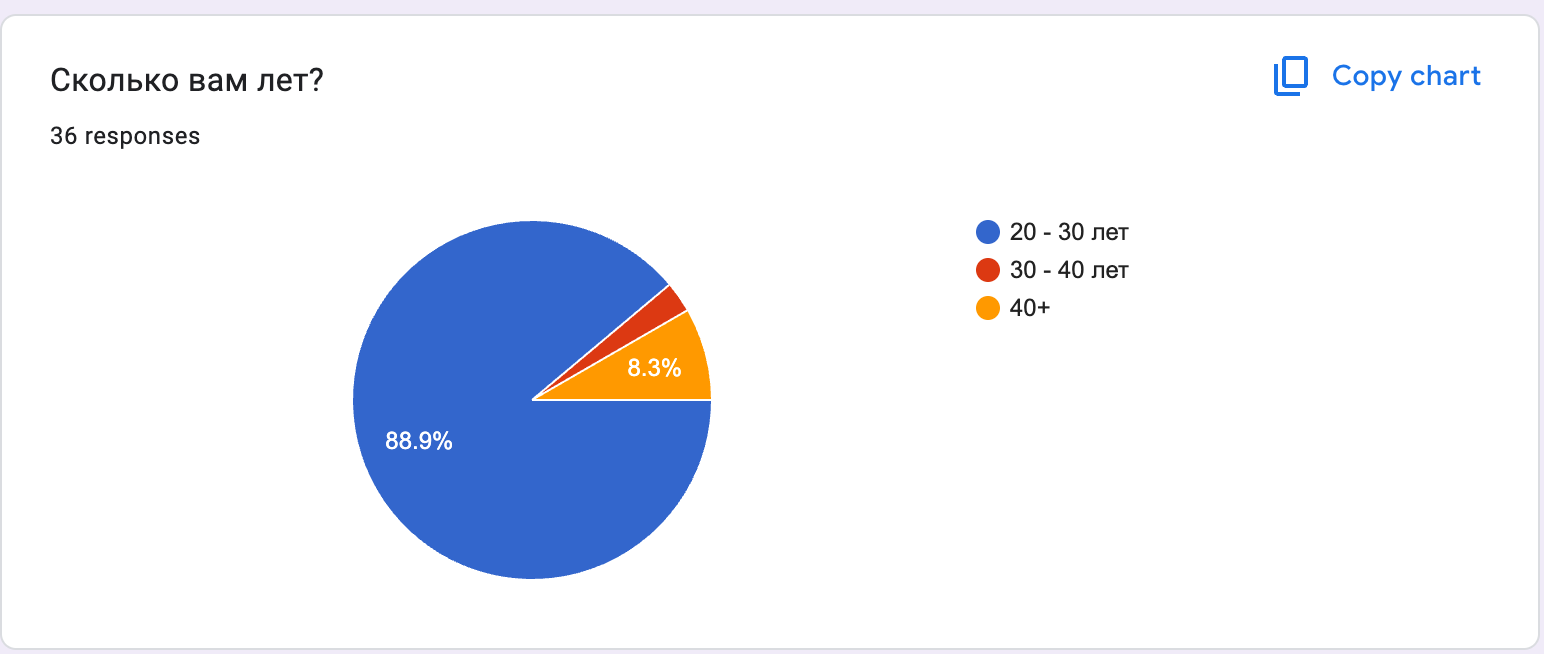
\includegraphics[width=0.8\linewidth]{images/pool/question_1.png}
    \captionof{figure}{Результаты демографии.}
    \label{fig:enter-label}
}

Касаемо профессии, больше половины принявших участие респондентов являются частными репетиторами. На 2 месте по частоте - преподаватели частных школ.

{
    \centering
    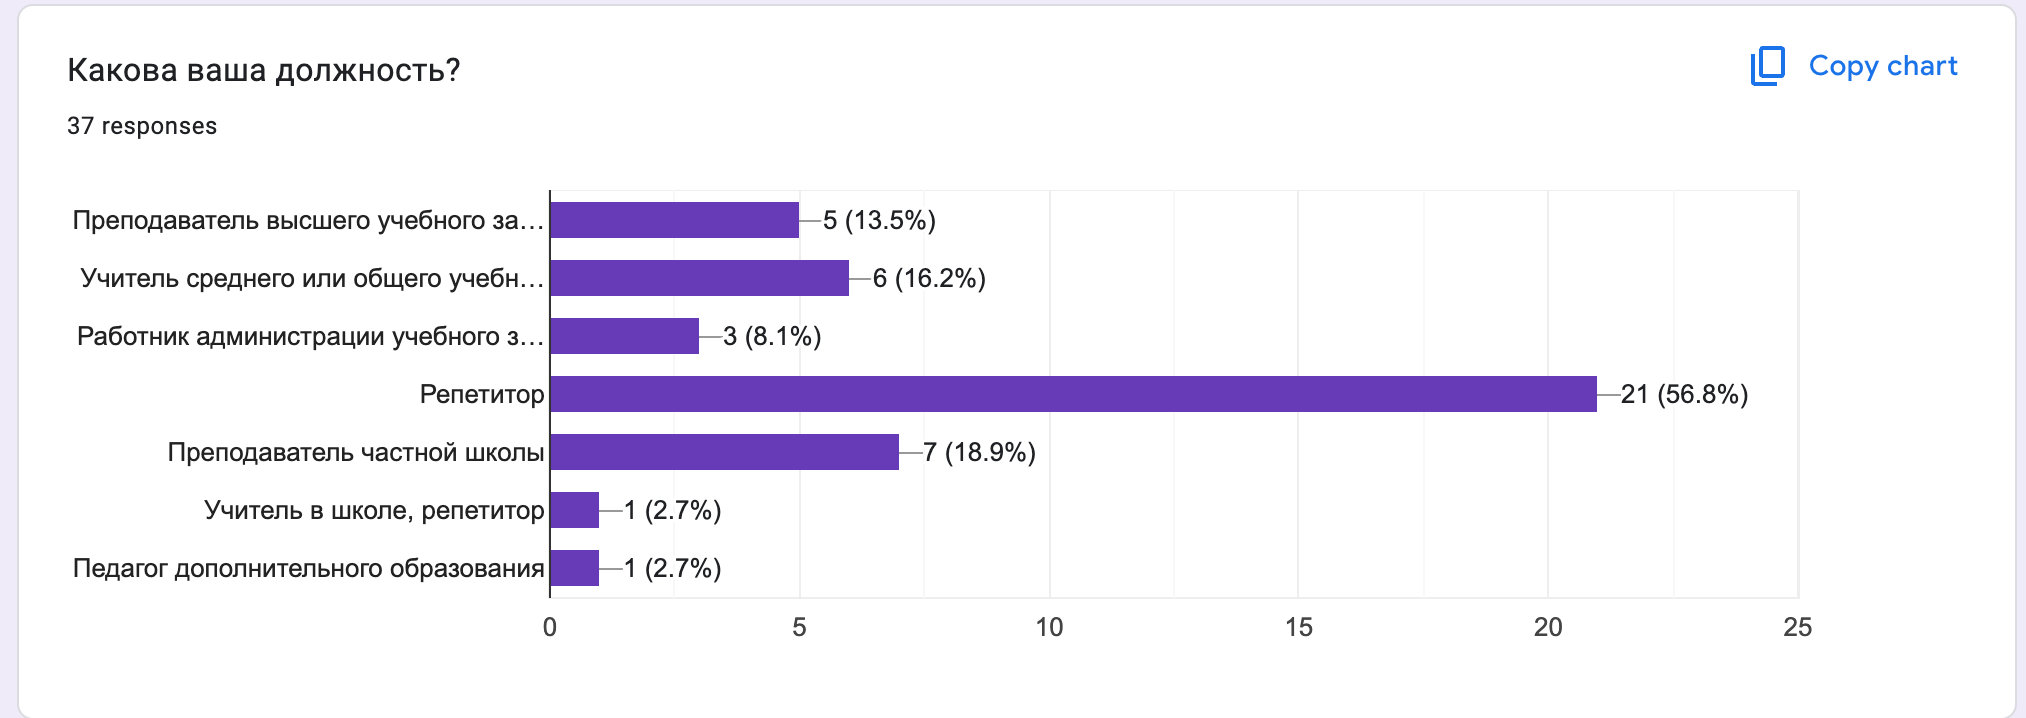
\includegraphics[width=0.8\linewidth]{images/pool/question_2.png}
    \captionof{figure}{Статистика по профессии.}
    \label{fig:enter-label}
}

Благодаря этой метрике, можно сегментировать ответы и определить в какой сфере самые популярные трудности. 

Далее, следующий вопрос направлен на выявление опытности респондента в сфере образования.  В результате 45.9\% опрошенных имеют опыт от 2 до 5 лет, 40.5\% только начинают свой путь в образовательной деятельности, и лишь 13\% опрошенных имеют более серьезный опыт.
{
    \centering
    \fbox{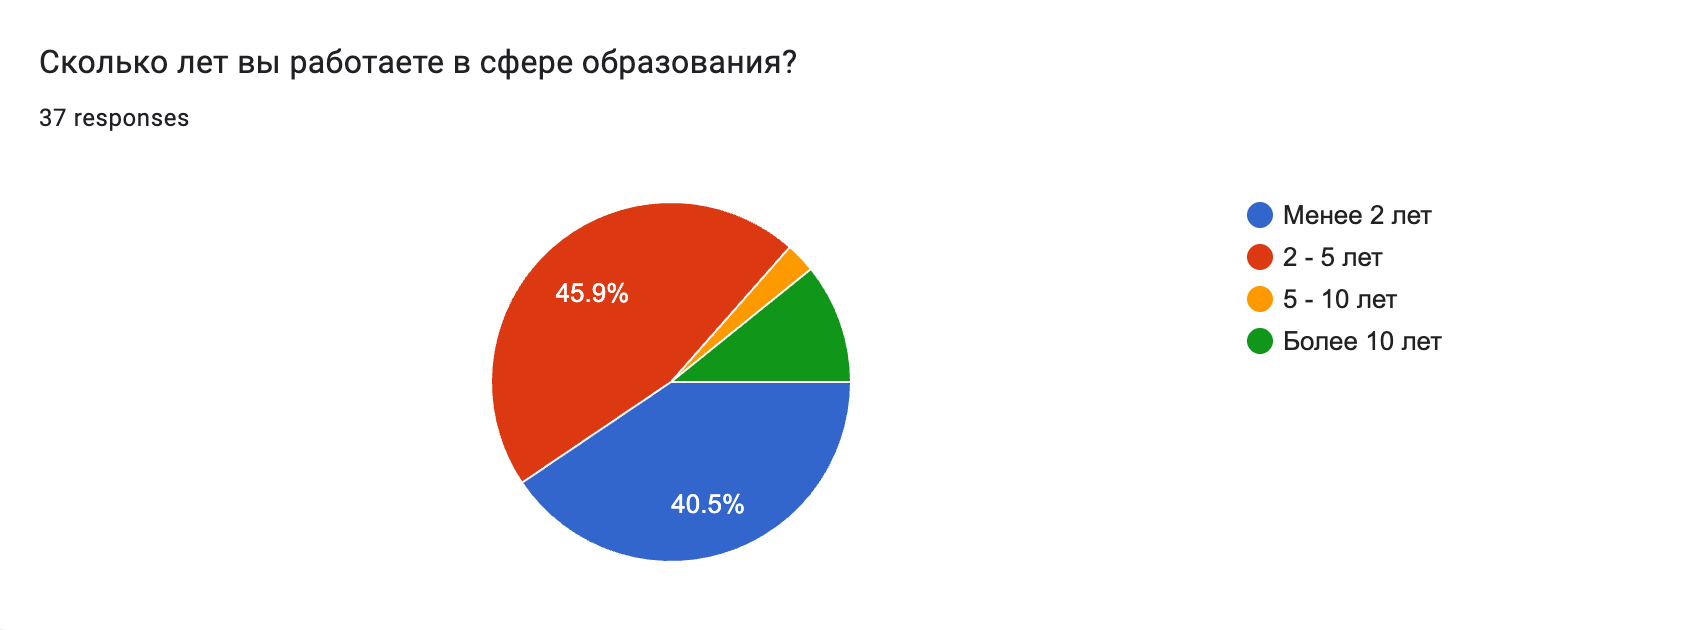
\includegraphics[width=0.8\linewidth]{images/pool/question_3.png}}
    \captionof{figure}{Опыт респондентов.}
    \label{fig:enter-label}
}

Следующий вопрос был направлен на выяснение самых времязатратных задач в работе респондентов.

Из рисунка 4 можно сделать вывод о том, что самой времязатратной задачей являетсяя загрузка учебных материалов, составление и корректировка расписания и коммуникация с учениками. Также из общей таблицы ответом можно получить ифномацию о том, что с проблемой загрузки учебных материалов сталкиваются в основном репетиторы, когда с проблемой коммуникации сталкиваются в основном учителя среднего образования, а учет посещаемости является главной проблемой преподавателей частных школ. Это говорит о том, что эти процессы требуют автоматизации.

{
    \centering
    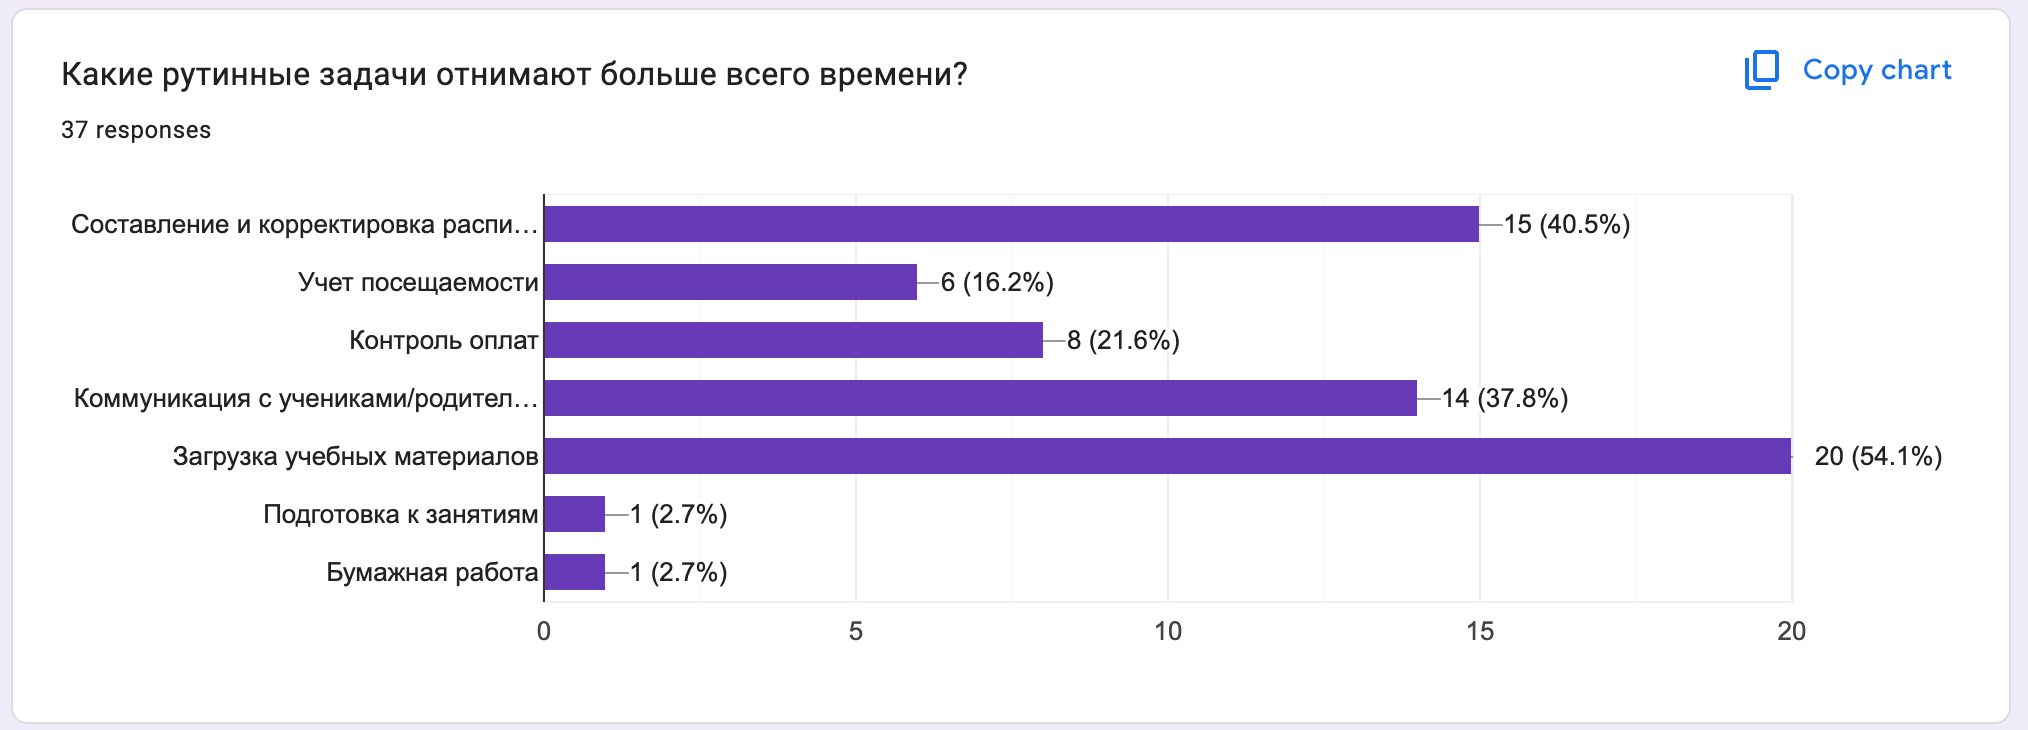
\includegraphics[width=0.8\linewidth]{images/pool/question_4.png}
    \captionof{figure}{Самые времязатратные задачи.}
    \label{fig:enter-label}
}

На рисунке 5 представлены результаты вопроса, направленного на выявление инструментария, которым пользуются респонденты сейчас для решения своих повседневных задач. 

{
    \centering
    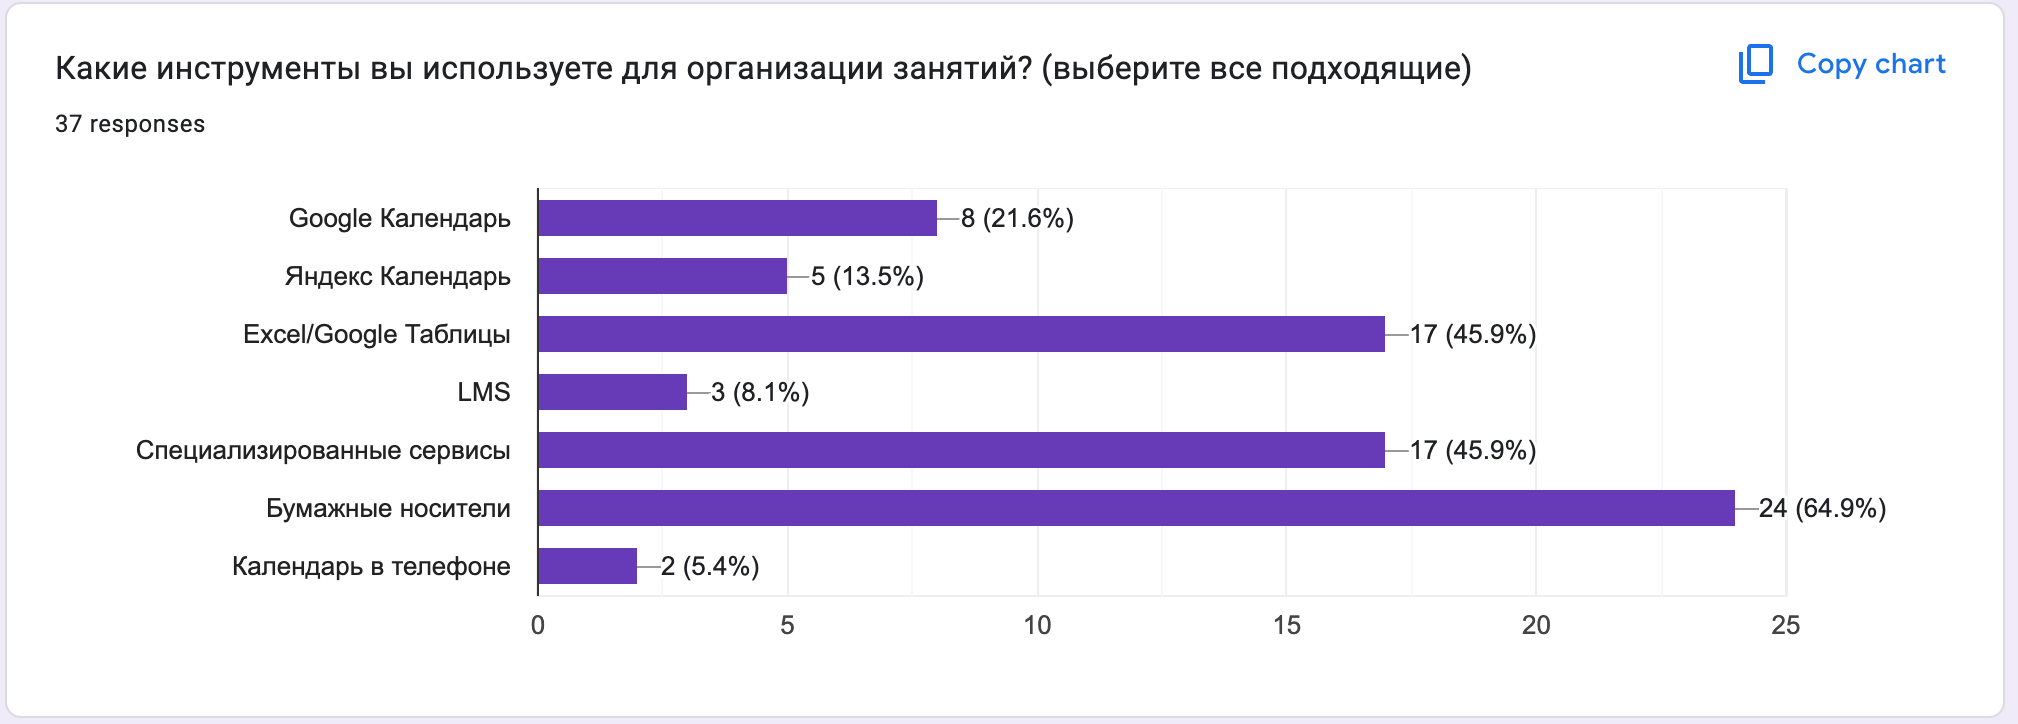
\includegraphics[width=0.8\linewidth]{images/pool/question_5.png}
    \captionof{figure}{Наиболее используемые инструменты}
    \label{fig:enter-label}
}

Из ответов вижно, что 64\% опрошенных предпочитают вести учет своей деятельности на бумаге и лишь 35\% предпочитают использовать электронные носители. Это дает сигнал о том, что многие респонденты не готовы использовать специализированные сервисы, поскольку, как показано на рисунке 7, эти же респонденты, что выбрали основной инструмент - бумагу, ответили, что главной их проблемой является дублирование и потеря информации. Исходя из этого можно сделать вывод о том, что эта часть целевой аудитории желает перейти от традиционног ведения учета на бумаге к более подходящему решению и испытывает трудности.

Также, из рисунка 5 можно сделать простой вывод о том, что хоть 45\% ответили, что используют специлизированные сервисы, также используют Excel. Это говорит о фрагментации данных. Респонденты вынуждены использовать множество сервисов одновременно и это подтверждает нишу моего решения.

На рисунке 6 представлен вопрос о владения компьютером. 

{
    \centering
    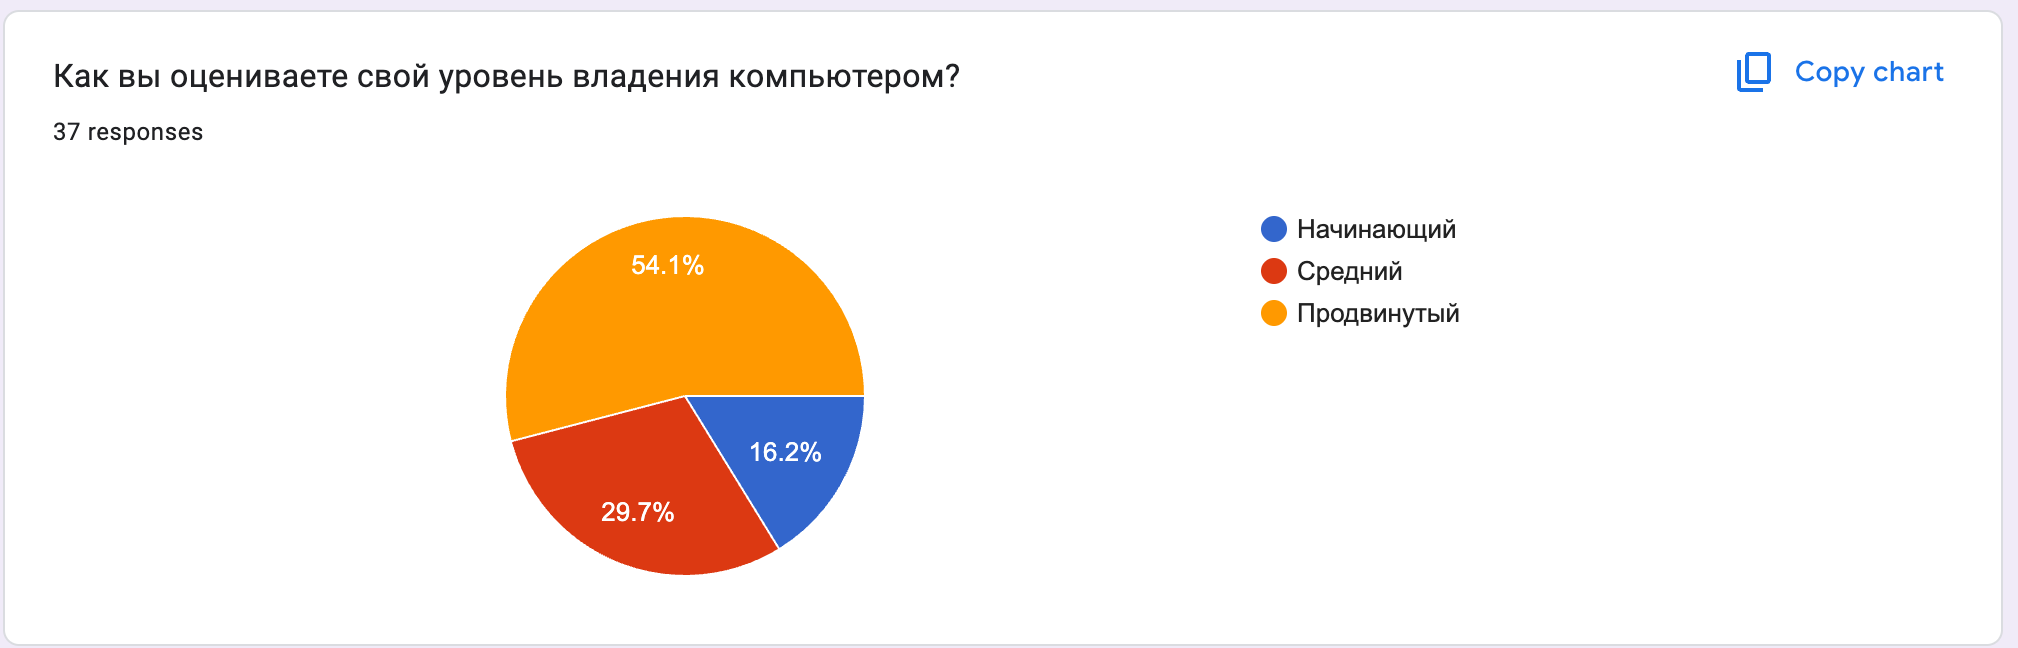
\includegraphics[width=0.8\linewidth]{images/pool/question_6.png}
    \captionof{figure}{Уровень владения компьютером.}
    \label{fig:enter-label}
}
Из результатов вопроса можно уверенно сказать, что основная часть целевой аудитории имеют высокий или средний уровень владения компьютером. Это значит, что интерфейс системы должен быть интутивно понятным и не вызывать большой когнитивной нагрузки.

Вопрос 7 нацелен на выявление удовлетворенности целевой аудитории с сервисами, которые они используют сейчас.

{
    \centering
    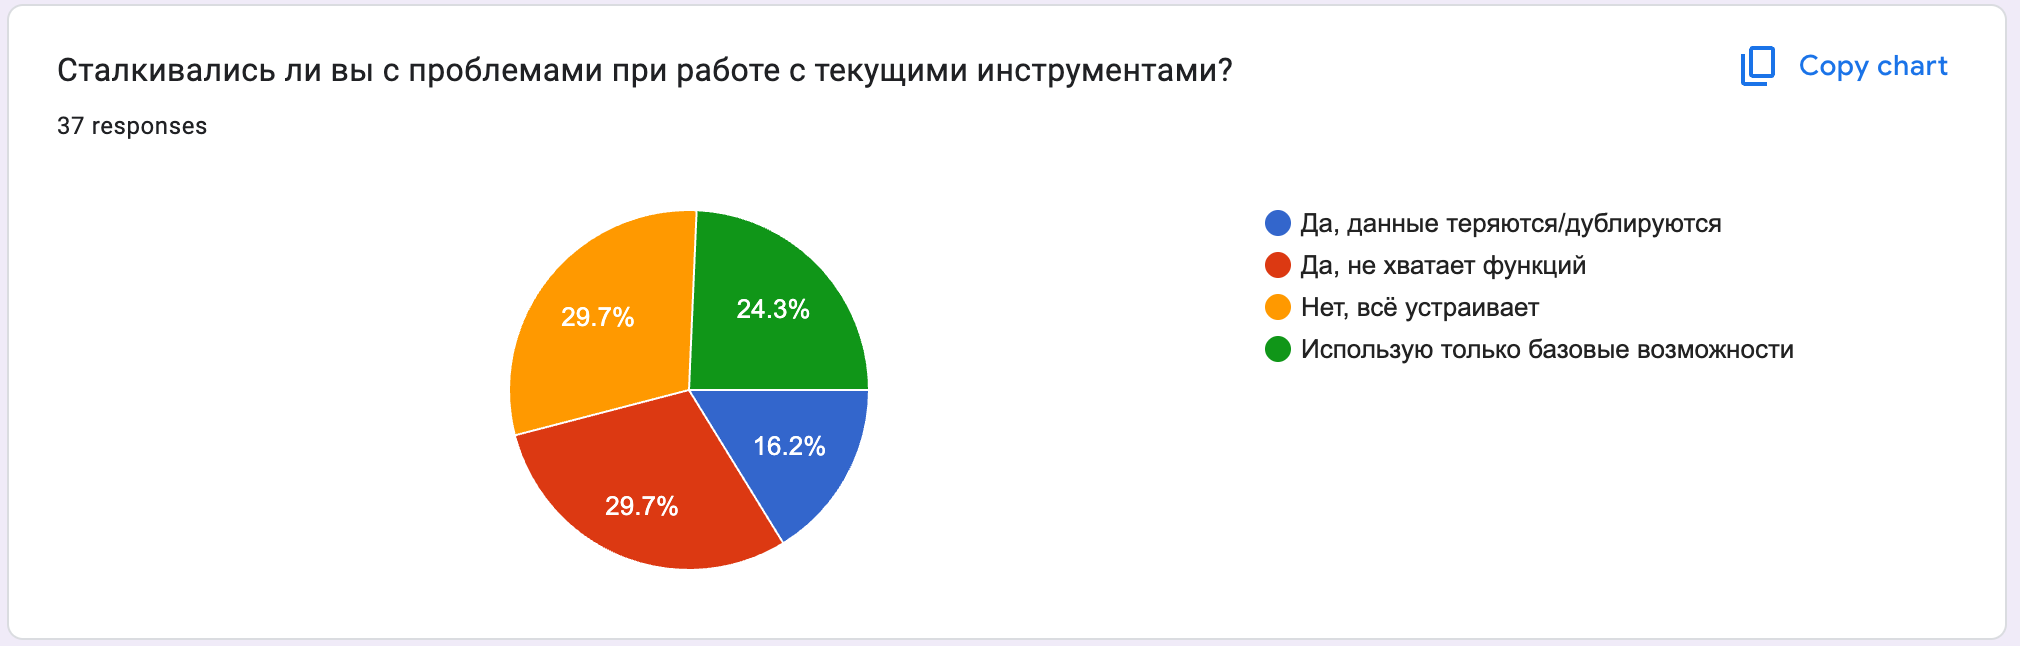
\includegraphics[width=0.8\linewidth]{images/pool/qustion_7.png}
    \captionof{figure}{Удовлетворенность текущими решениями.}
    \label{fig:enter-label}
}

Здесь видно, что мнения респондентов разделились. Около трети респондентов ответили, что им не хватает некоторого функционала, 16\% заявлили им не хватает критически важного функционала и испытывают проблемы с хранением информации. Это дает основание полагать, что мое решение будет особенно актуально для минимизирования ручного труда.

По итогам 8 вопроса, представленного на рисунке 8, можно сделать вывод о том, что весь перечисленный функционал востребован среди целевой аудитории. Из сводной таблицы, можно сделать вывод о том, что те респонденты, которые указали своей главной проблемой "Составление и корректировка расписания", использующие Excel больше всего выбрали желаемый функционал "Автоматическое расписание с повторяемыми занятиями", а также "Ведение финансовой отчетности". 
Также, те респонденты, уровень владения компьютером которых явлется низким или средним, ответили, что хотели бы видеть адаптированную версию сервиса под мобильные устройства.
А гибкие настройки доступа, разделение групп обучающихся на открытые и закрытые, отметили в основном репетиторы и преподаватели частных школ и заведений.

{
    \centering
    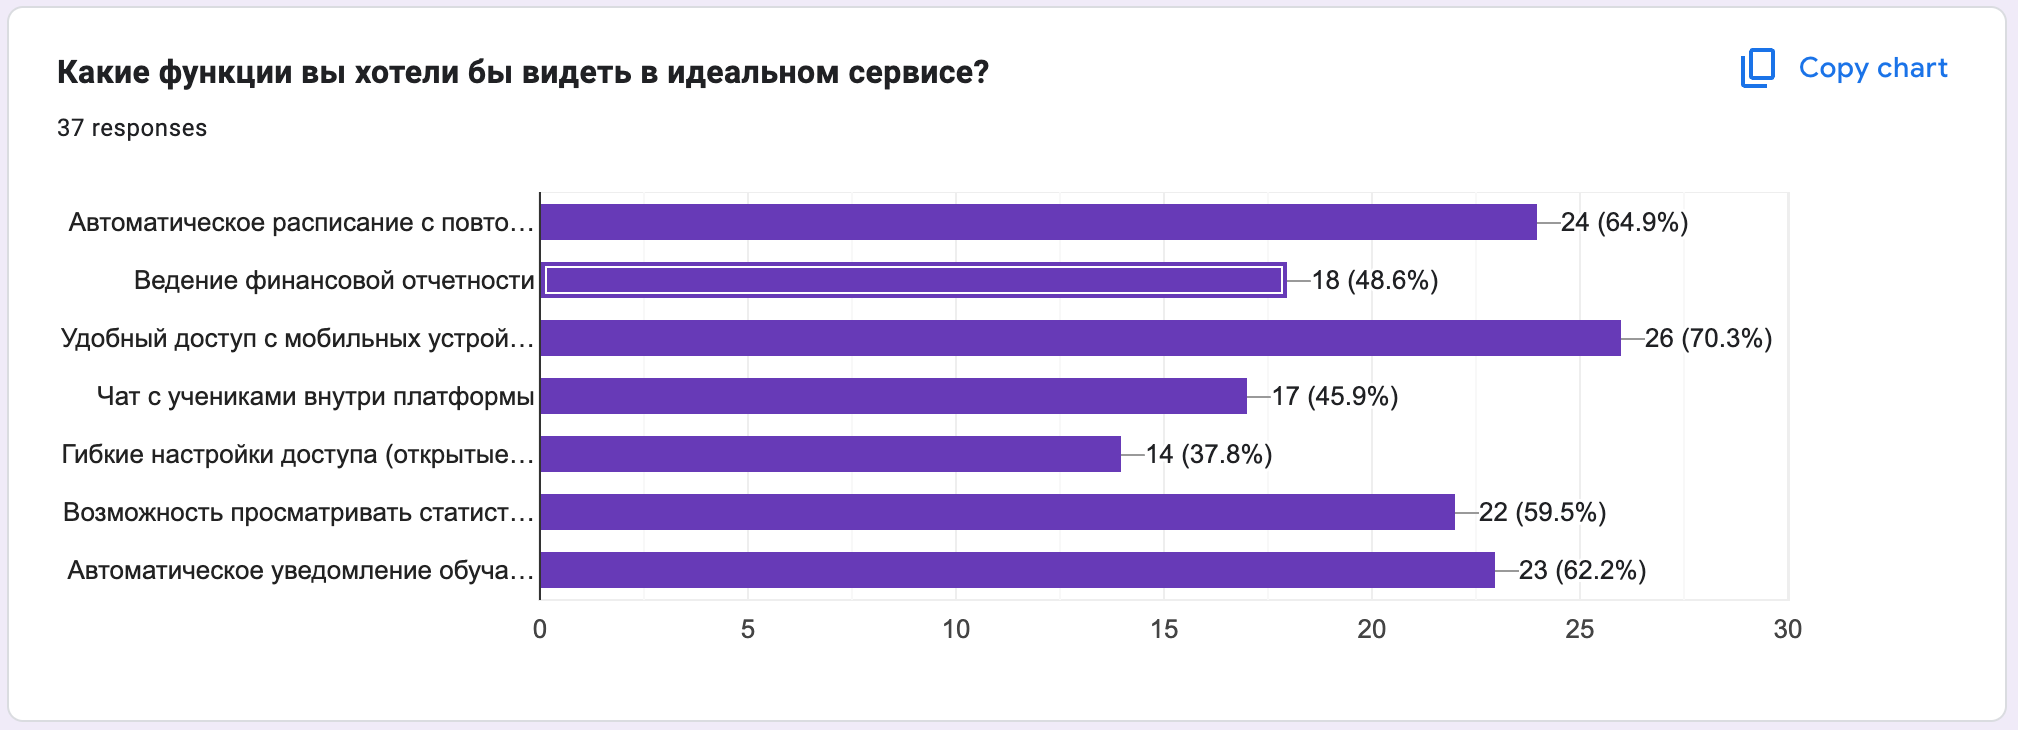
\includegraphics[width=0.8\linewidth]{images/pool/question_8.png}
    \captionof{figure}{Функции идеального сервиса}
    \label{fig:enter-label}
}


Из результатов проведенного опроса, можно составить портрет среднестистического пользователя системы администирования групповых занятий. 
 
Портрет ЦА:
\begin{itemize}
    \item возраст: 25–35 лет;
    \item опыт работы: 2-10 лет;
    \item техническая подготовка: средний уровень.
Многие не имеют опыта работы с профессиональными CRM или LMS, но активно используют базовые инструменты (Яндекс Календарь, Excel, мессенджеры).
\end{itemize}

Потребности:

\begin{itemize}
    \item быстрое создание групп и расписаний без ручного ввода данных;
    \item учет посещаемости с возможностью отметки в реальном времени;
    \item автоматический расчет доходов;
    \item доступ к статистике (посещаемость, оплаты, успеваемость);
\end{itemize}

Проблемы, с которыми сталкиваются:

\begin{itemize}
    \item фрагментация инструментов: расписание в одном месте, оплаты — в другом, общение — в мессенджере;
    \item сложности с контролем задолженностей учеников;
    \item отсутствие единого пространства для работы с группами;
    \item недостаток коммуникации с обучающимися.
\end{itemize}

Также, для автоматизации процесса ведения груп, а также расширения функциональности системы, проанализирована вторичная аудитория: обучающиеся.

Портрет ЦА:

\begin{itemize}
    \item возраст обучающихся: 12–25 лет
    \item техническая подготовка: средняя. Хорошо владеют компьютером и телефоном, но не имеют навыков работы в профессиональных CRM системах и LMS
\end{itemize}

Потребности:

\begin{itemize}
    \item просмотр расписания занятий и домашних заданий;
    \item запись на групповые или индивидуальные занятия;
    \item доступ к истории оплат и посещаемости.
\end{itemize}

Проблемы, с которыми сталкиваются:

\begin{itemize}
    \item необходимость уточнять расписание у преподавателя;
    \item отсутствие прозрачности в оплатах.
\end{itemize}

\mysubsection{Анализ требований целевой аудитории}

По сформерованным портретам основной целевой аудитории можно определиться с списоком функциональных и нефункциональных требований к системе, которые будут нацелены на улучшение пользовательского опыта и решение главных задач целевой аудитории.


\mysubsection{Анализ аналогов и конкурентов}

К сожалению, сегодня, большинство преподавателей и репетиторов предпочитают использовать excel таблицы.
Преимущества:
\begin{itemize}
    \item Приемственность. 
    
    Многие используют Excel поскольку десятилетиями использовали его для выполнения всех своих рутинных задач и попросту не хотят переходить на что-то более новое.
    \item Доступность. 
    
    Excel предустановлен на всех Windows устройствах и доступен сразу "из коробки". Пользователю сразу доступен весь функционал.
    \item Удобство хранения. 
    
    Некоторые xslx редакторы поддерживают облачное хранение, обеспечивая своим пользователем общим доступом с разных устройств, лишая их необходимости носить устройства накопления информации.
\end{itemize}
Недостатки:
\begin{itemize}
    \item Сбор информации. 
    
    Пользователю необхожимо вручную вводить информацию по каждому своему ученику на каждое занятие. На это тратится много времени, а также много теряется на построение коммуникации вне системы.
    \item Отсутствие целевой направленности. 
    
    Изначально excel не строился как платформа для моей целевой аудитории, а следственно не может учитывать их потребности. 
    \item Переполненость функционалом. 
    
    Excel редактор представляет собой многофункциональное приложение, способности которого только затрудняют навигацию по приложению, отвлекая тем функционалом, который не требуется для достижения целей ЦА.
\end{itemize}

Из опроса, был выявлен неочевидный, но распространенный инструмент: бумажные носитель.

Преимущества:
\begin{itemize}
    \item доступность;
    
Блокнот илил ежедневник, как правило, всегда под рукой у преподавателя.
    \item простота использования;
    
Поскольку писать могут абсолютно все, вести учет и заметки можно в любом виде.
\end{itemize}
Недостатки:
\begin{itemize}
    \item ненадежность;
    
Бумага - материал легко воспламенимый и подвержен влаге. Его крайне легко испортить, а значит быстро утратить важную ифнормацию
    \item времязатратность.
    
Ведение ежедневника обязывает тратить значительное время на орагнизацию и структуризацию данных. Это является главным недостатком, поскольку это время сегодня - главный ресурс.

\end{itemize}

Ярепетитор - прямой конкурент моей платформе, который предоставляет общий функционал создания занятий, просмотра расписания, учета заработка и оплаченных часов.
Однако, эта платформа обладает главным недостатком - односторонность использования. 
Система предоставляет функционал только для преподавателя.

Преимущества:
\begin{enumerate}
    \item Наличие календаря и вохможность вести расписание.
    \item Возможность вести статистику заработка.
    \item Многоплатформенность.
    
Сервис доступен как в веб версии, так и android и IOS приложение;
    \item наличие файлаобменника.
    
Сервис предоставляет возможность хранения заданий и материалов к занятиям.
    \item интеграция с сторонними сервисами. 
    
Сервис поддержвает авторизацию черех Google и Apple аккаунты.
\end{enumerate}

Недаостатки:
\begin{enumerate}
    \item Пользователю приходится вручную заносить каждого своего ученика в систему, а также всю информацию о нем.
    \item Пользователю приходится самому уведомлять своих учениках о переносе занятия
    \item Ученики пользователя не имеют возможности получить общую информацию о курсах и занятиях преподавателя без предварительной коммуникации. 
    
Это пораждает лишнее потраченное время на согласование времени, цены и условия проведения занятий. 
    \item Сложный и неинтуитивный интерфейс, затрудняющий использования расписания и создание занятий (рисунок 10).
\end{enumerate}

{
    \centering
    
\includegraphics[width=0.5\linewidth]{analog1.jpg}
    \captionof{figure}{Пример интерфейса аналога}
    \label{fig:enter-label}
}

Исходя из анализа конкурентов, можно выделить следующие преимущества разрабатываемого решения:

\begin{enumerate}
    \item Специализация на групповых занятиях:

Инструменты заточены под нужды преподавателей: быстрое создание групп, массовая отметка посещаемости.

    \item Все в одном месте:

Объединение расписания, оплат, коммуникации и контента избавляет от необходимости переключаться между сервисами.

    \item  Простота для не технических пользователей:

Минимум настроек, интуитивные формы, подсказки при первом входе.

    \item Финансовая прозрачность:

Автоматические напоминания об оплате, статистика доходов/расходов.

\end{enumerate}



\mysubsection{Функциональные и не функциональные требования}

Перед тем как приступить к проектированию системы, необходимо выявить все функицональные и нефункциональные требования, представленные к системе на основе опроса и конкурентов. Полученные требования отражают фактический функционал и технические особенности системы. Они включают в себы сильные стороны используемых аналогов, а также стремятся исключить повторения недостатков конкурентов.

\mysubsubsection{Функциональные требования}
Общие функциональные требования представлены на UML диаграмме 
\hypertarget{pi10}{\hyperlink{pic10_text}{рисунке 10}}

{
    \centering
    \fbox{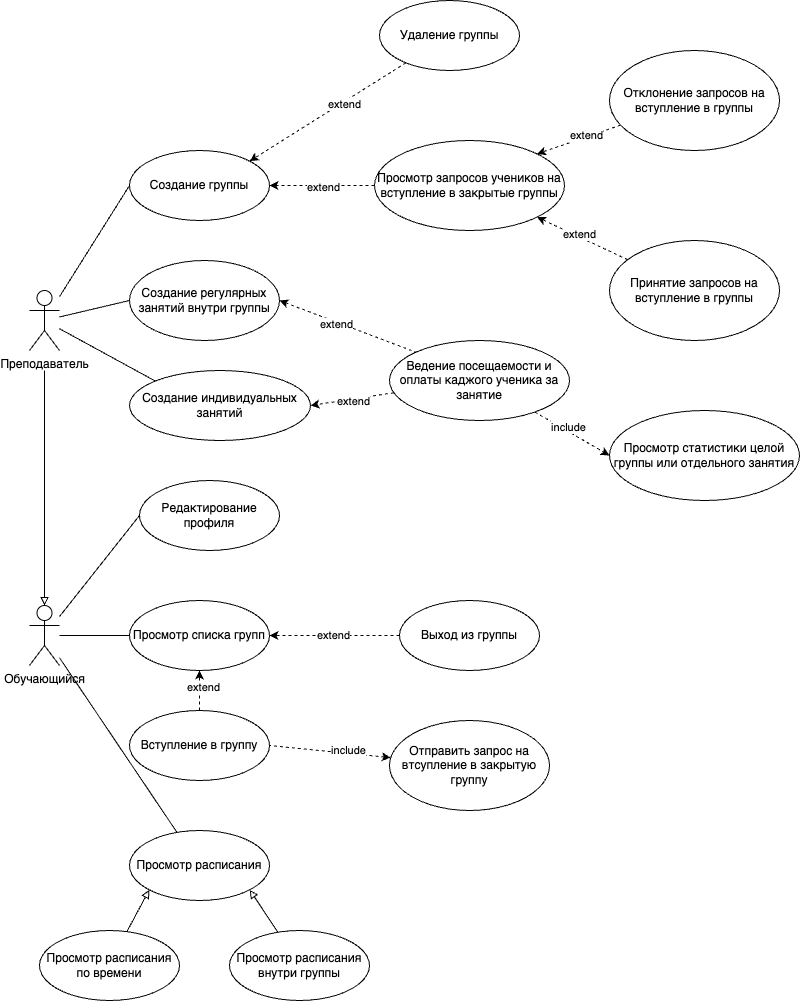
\includegraphics[scale=0.4]{images/UML.png}}
    \captionof{figure}{\hyperlink{pic10}{\hypertarget{pic10_text}{UML диаграмма по пользователям}}}
}



Для преподавателей:

\begin{enumerate}
    \item Создание групп с настройкой параметров (макс. количество учеников, стоимость занятий).
    \item Составление гибкого расписания: повторяющиеся и разовые занятия. Перенос занятий.
    \item Отметка посещаемости с возможностю добавления комменатриев.
    \item Возможность указать стоимость каждого занятия.
    \item Введение статистики по доходам.
    \item Управление контентом: добавление материалов к занятиям и домашнего задания.
    \item Уведомление учеников о переносах или отмены занятий.
\end{enumerate}

Для обучающихся:

\begin{enumerate}
    \item Личный кабинет с расписанием и историей посещений занятий.
    \item Вступление в группы преподавателей и просмотр открытых окон.
    \item Вомзожность поиска преподавателей.
\end{enumerate}

\mysubsubsection{Нефункциональные требования}

\begin{itemize}
    \item удобство интерфейса;

Современные паттерны применения дизайна, а также адаптивность под мобильные устройства
    \item безопасность;

Надежное хранение персональных данных.
    \item производительность;

Возможность посещения платформы более 1000 человек одновременно.
    \item подержкка внешних сервисов, таких как вход через Google или Yandex аккаунты.
\end{itemize}


\mysubsection{Проектирование}

Для проектирования бизнес процессов выбрана методология описания IDEF0. Она отлично подходит для ...

Бизнес процесс входа систему представлен на рисунке 11.

{
    \centering
    
\includegraphics[width=0.5\linewidth]{images/idef0/image.png}
    \captionof{figure}{Общий бизнес процесс входа в систему в нотации IDEF0.}
    \label{fig:enter-label}
}

Этот процесс декомпозируется на регистрацию и авторизацию на уровень декомпозиции 1 и представлен на рисунке 12.
\newpage

{
    \centering
    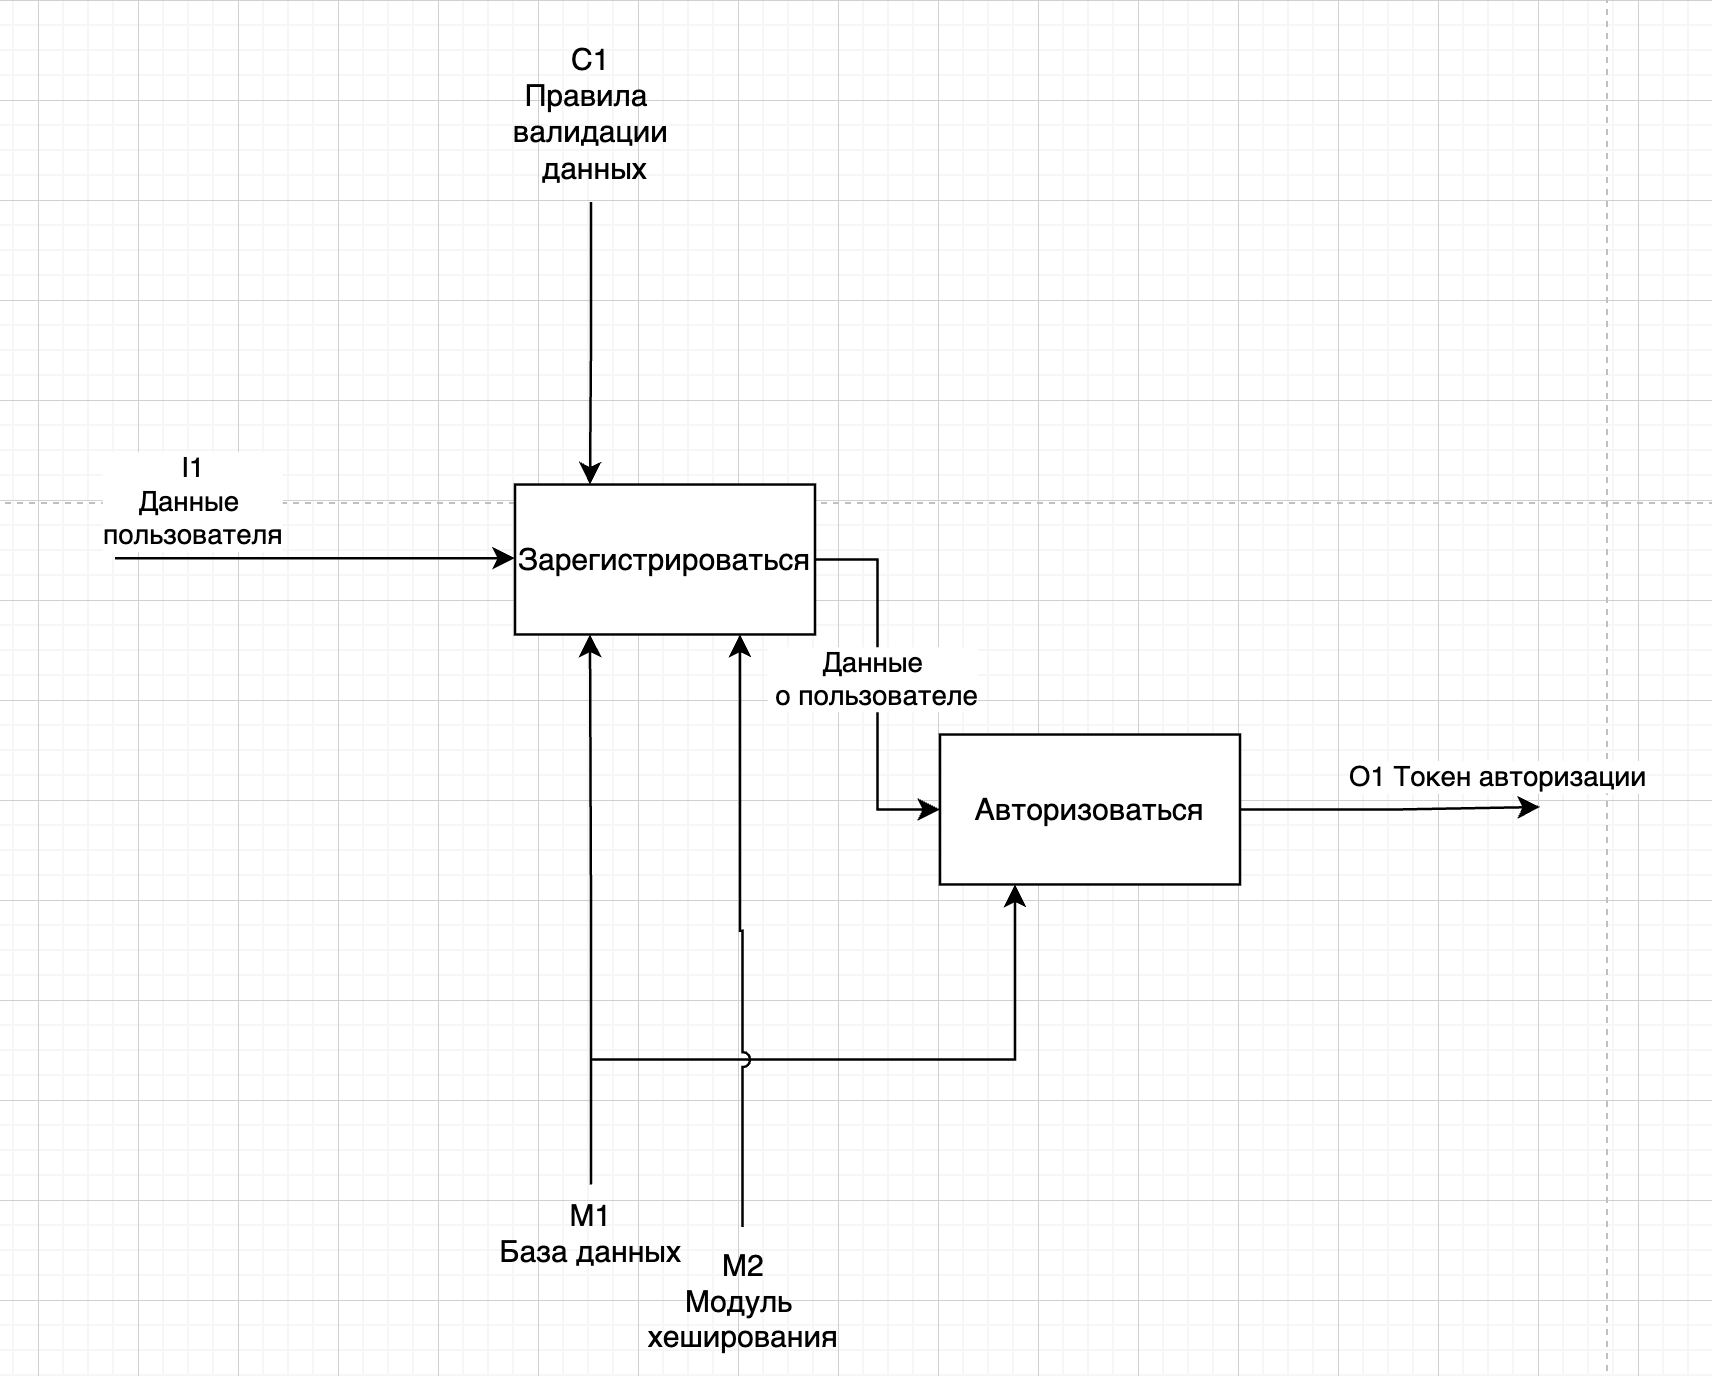
\includegraphics[width=0.5\linewidth]{images/idef0/image2.png}
    \captionof{figure}{Процесс входа в систему в нотации IDEF0 на 1 уровне декомпозиции.}
    \label{fig:enter-label}
}

Далее, рассмотрим процесс регистрации. Здесь, на вход поступают данные пользователя, а на выход id нового пользователя. Из механизмов здесь принимает участие модуль хеширования паролей, а также база данных в которой хранятся данные. Из правил, здесь присутствует Правила валидации полей

{
    \centering
    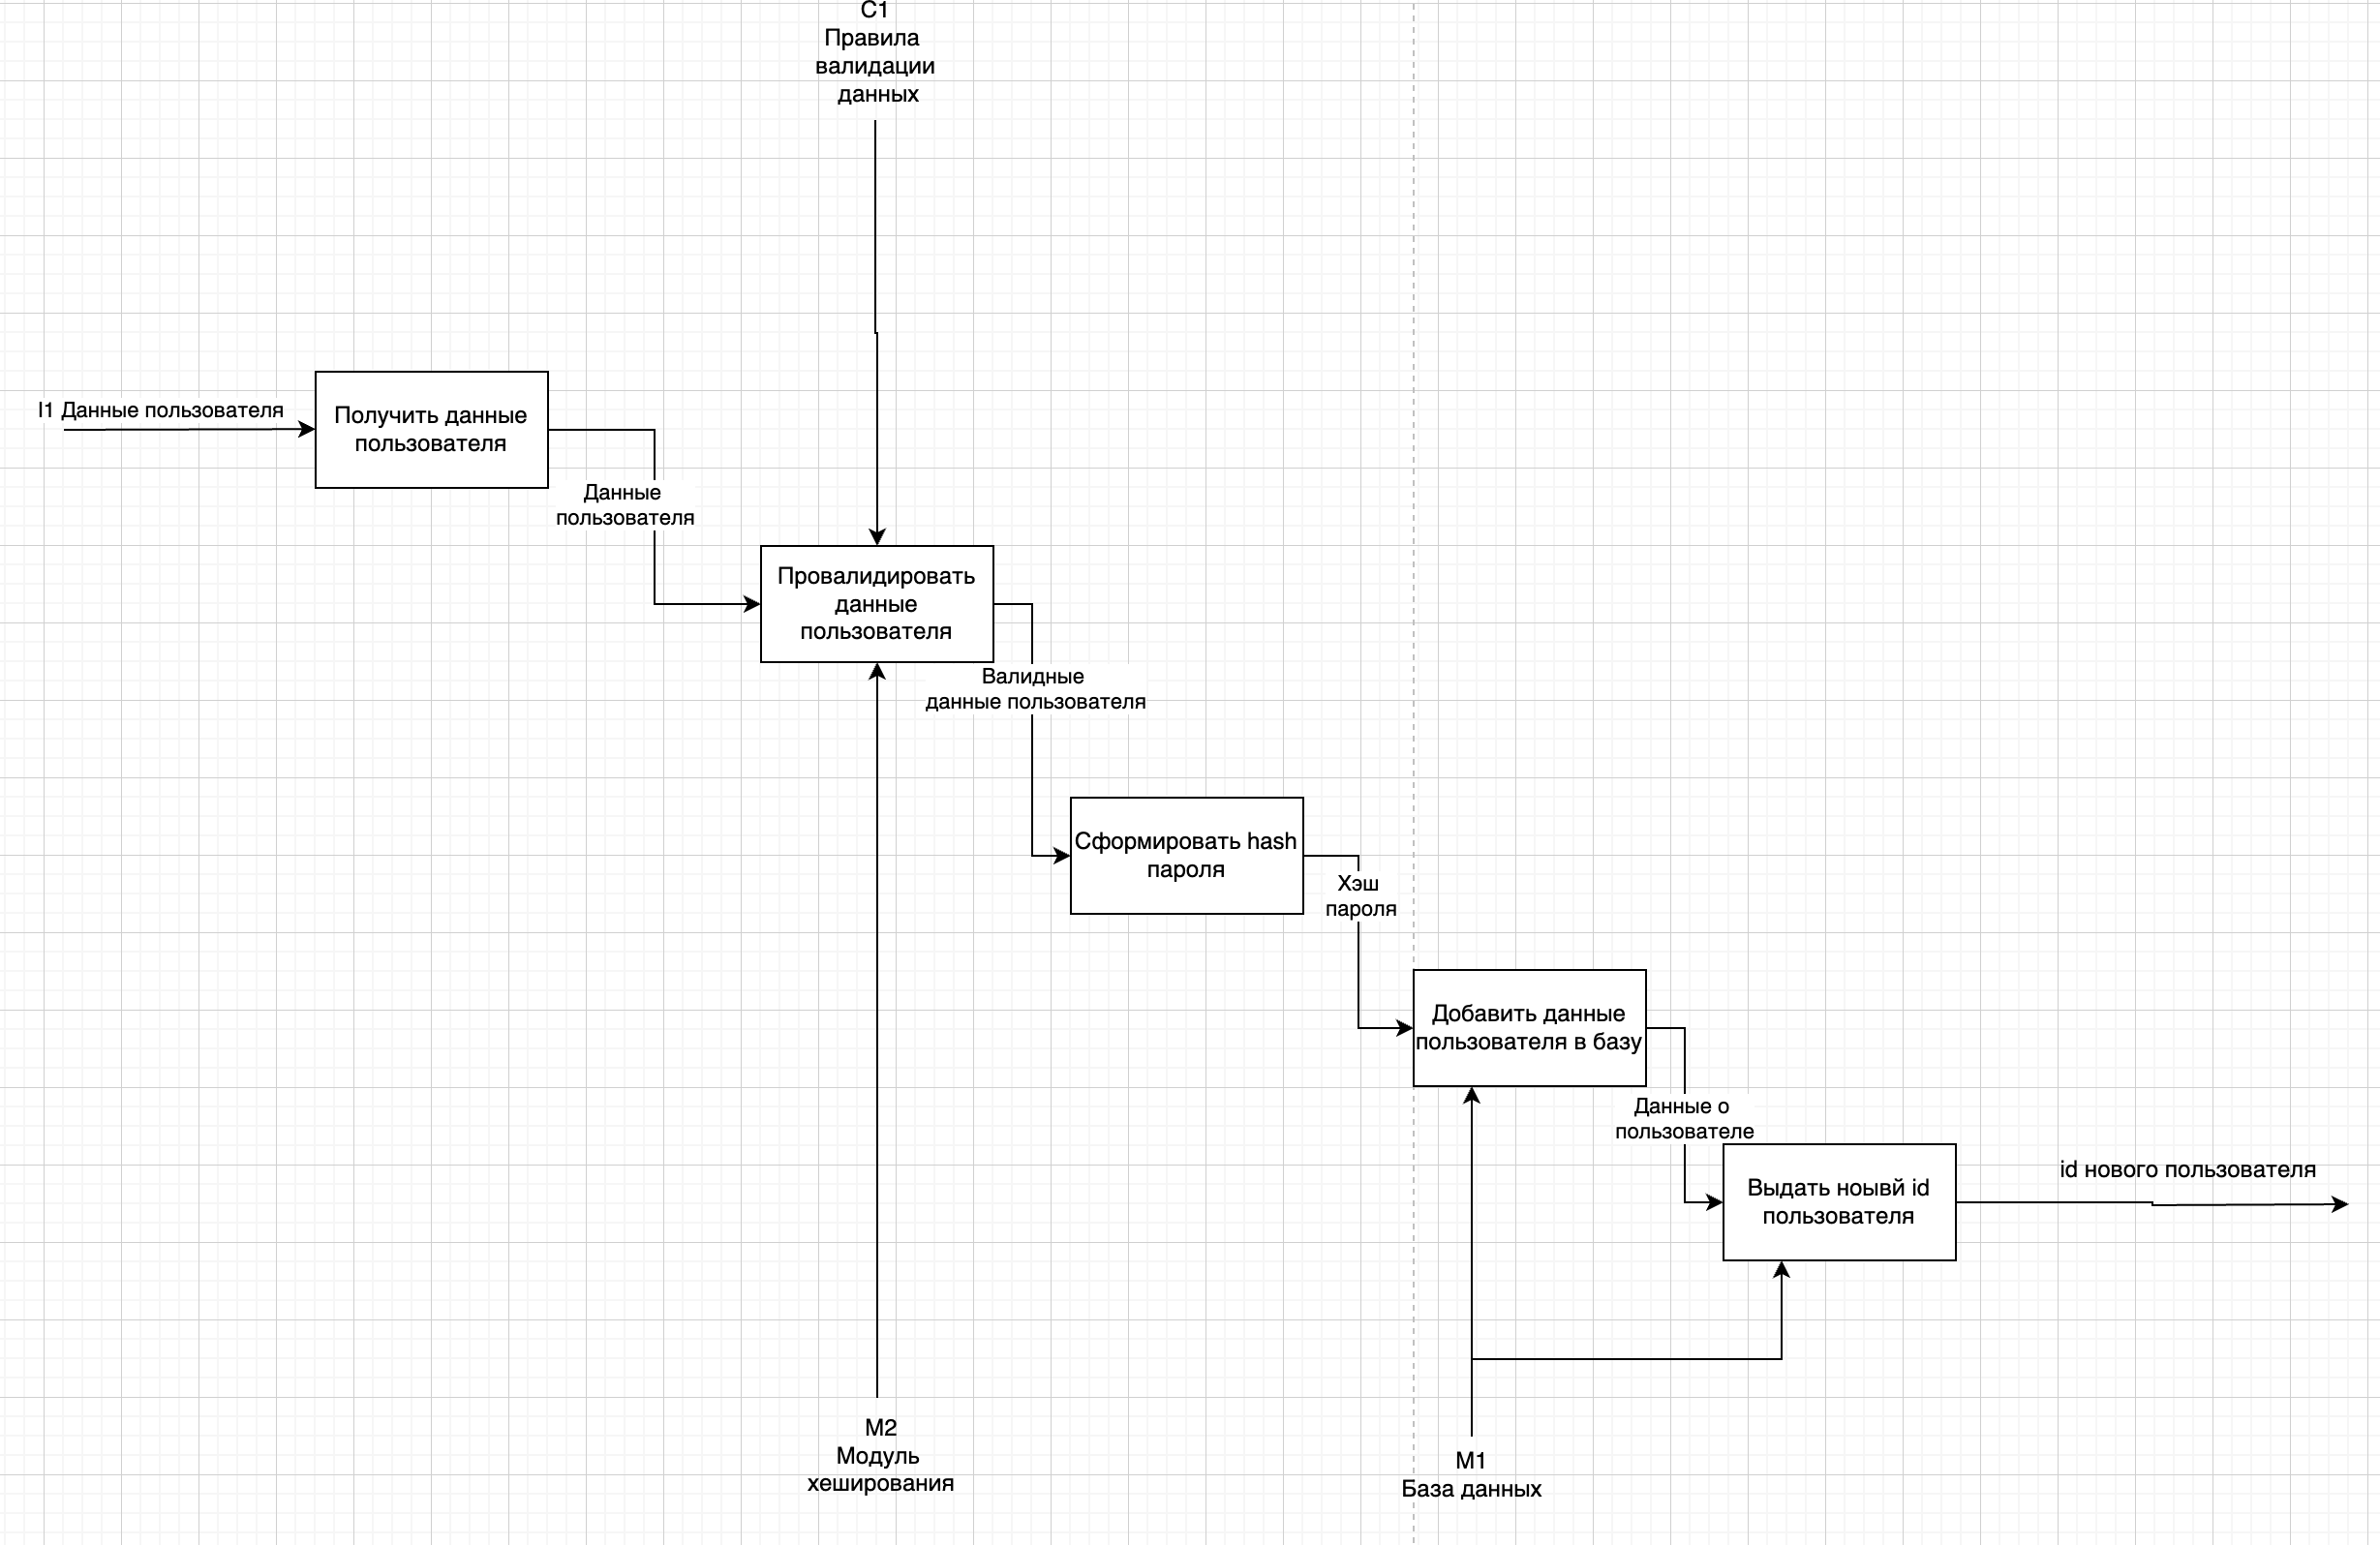
\includegraphics[width=0.7\linewidth]{images/idef0/image3.png}
    \captionof{figure}{Процесс регистрации пользователя в нотации IDEF0.}
    \label{fig:enter-label}
}

В процессе регистарции существует процесс валидации, декомпозированный на рисунке 14.

{
    \centering
    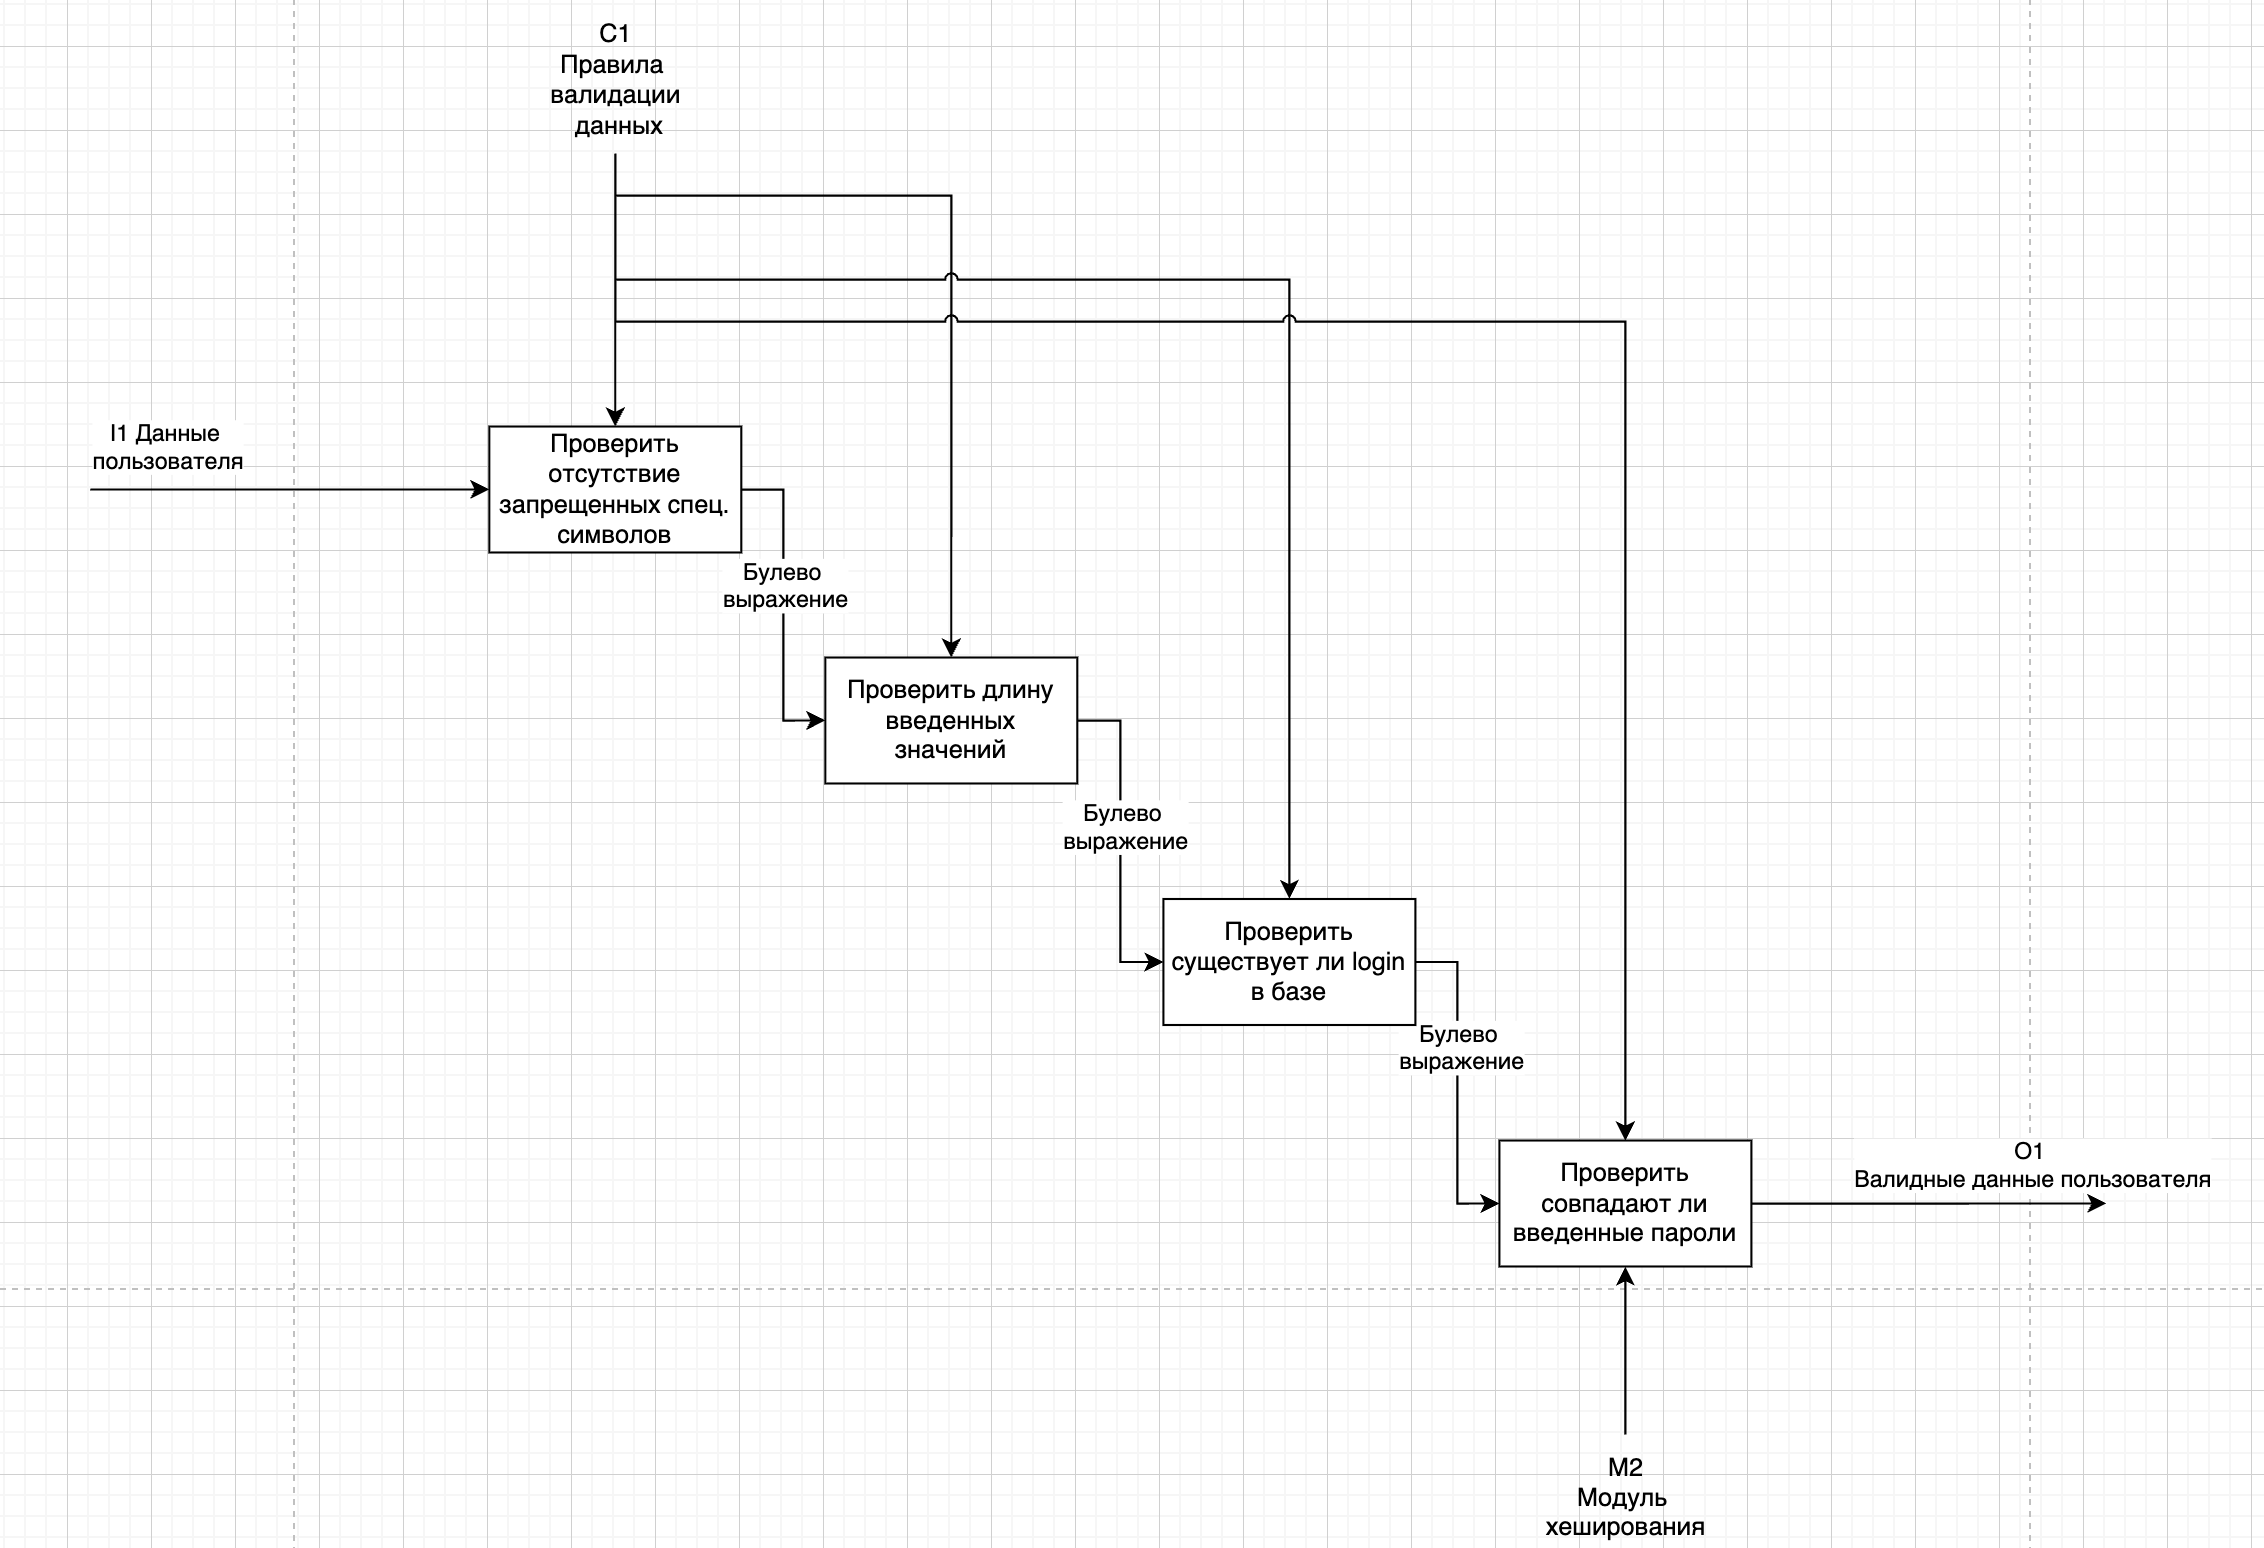
\includegraphics[width=0.7\linewidth]{images/idef0/image4.png}
    \captionof{figure}{Процесс валидации данных в нотации IDEF0.}
    \label{fig:enter-label}
}
Здесь данные сначала валидируется по типу данных (строки числа или другое), далее проверяется существование введенного логина в базе данных, а также сверяются введеные пароли. 

После того как пользователь зарегистрирован, ему необходимо авторизоваться под своим логином для доступа в систему. 

Доступ в систему ограничен специальным токеном авторизации, который пользователь получает по факту авторизации и имеет срок истечения. По истечению срока действия токена, пользователю необходимо заново авторизоваться. ( как правило это очень большой срок и необходимость повторой авторизации возникает при смене браузера или при очистке кеша браузера, поскольку этот токен хранится в локальном хранилище веб сайта).

В процессе авторизации, также используется процесс валидации введенных данных, после чего формируется уникальный идентификатор доступа в систему.

 {
     \centering
     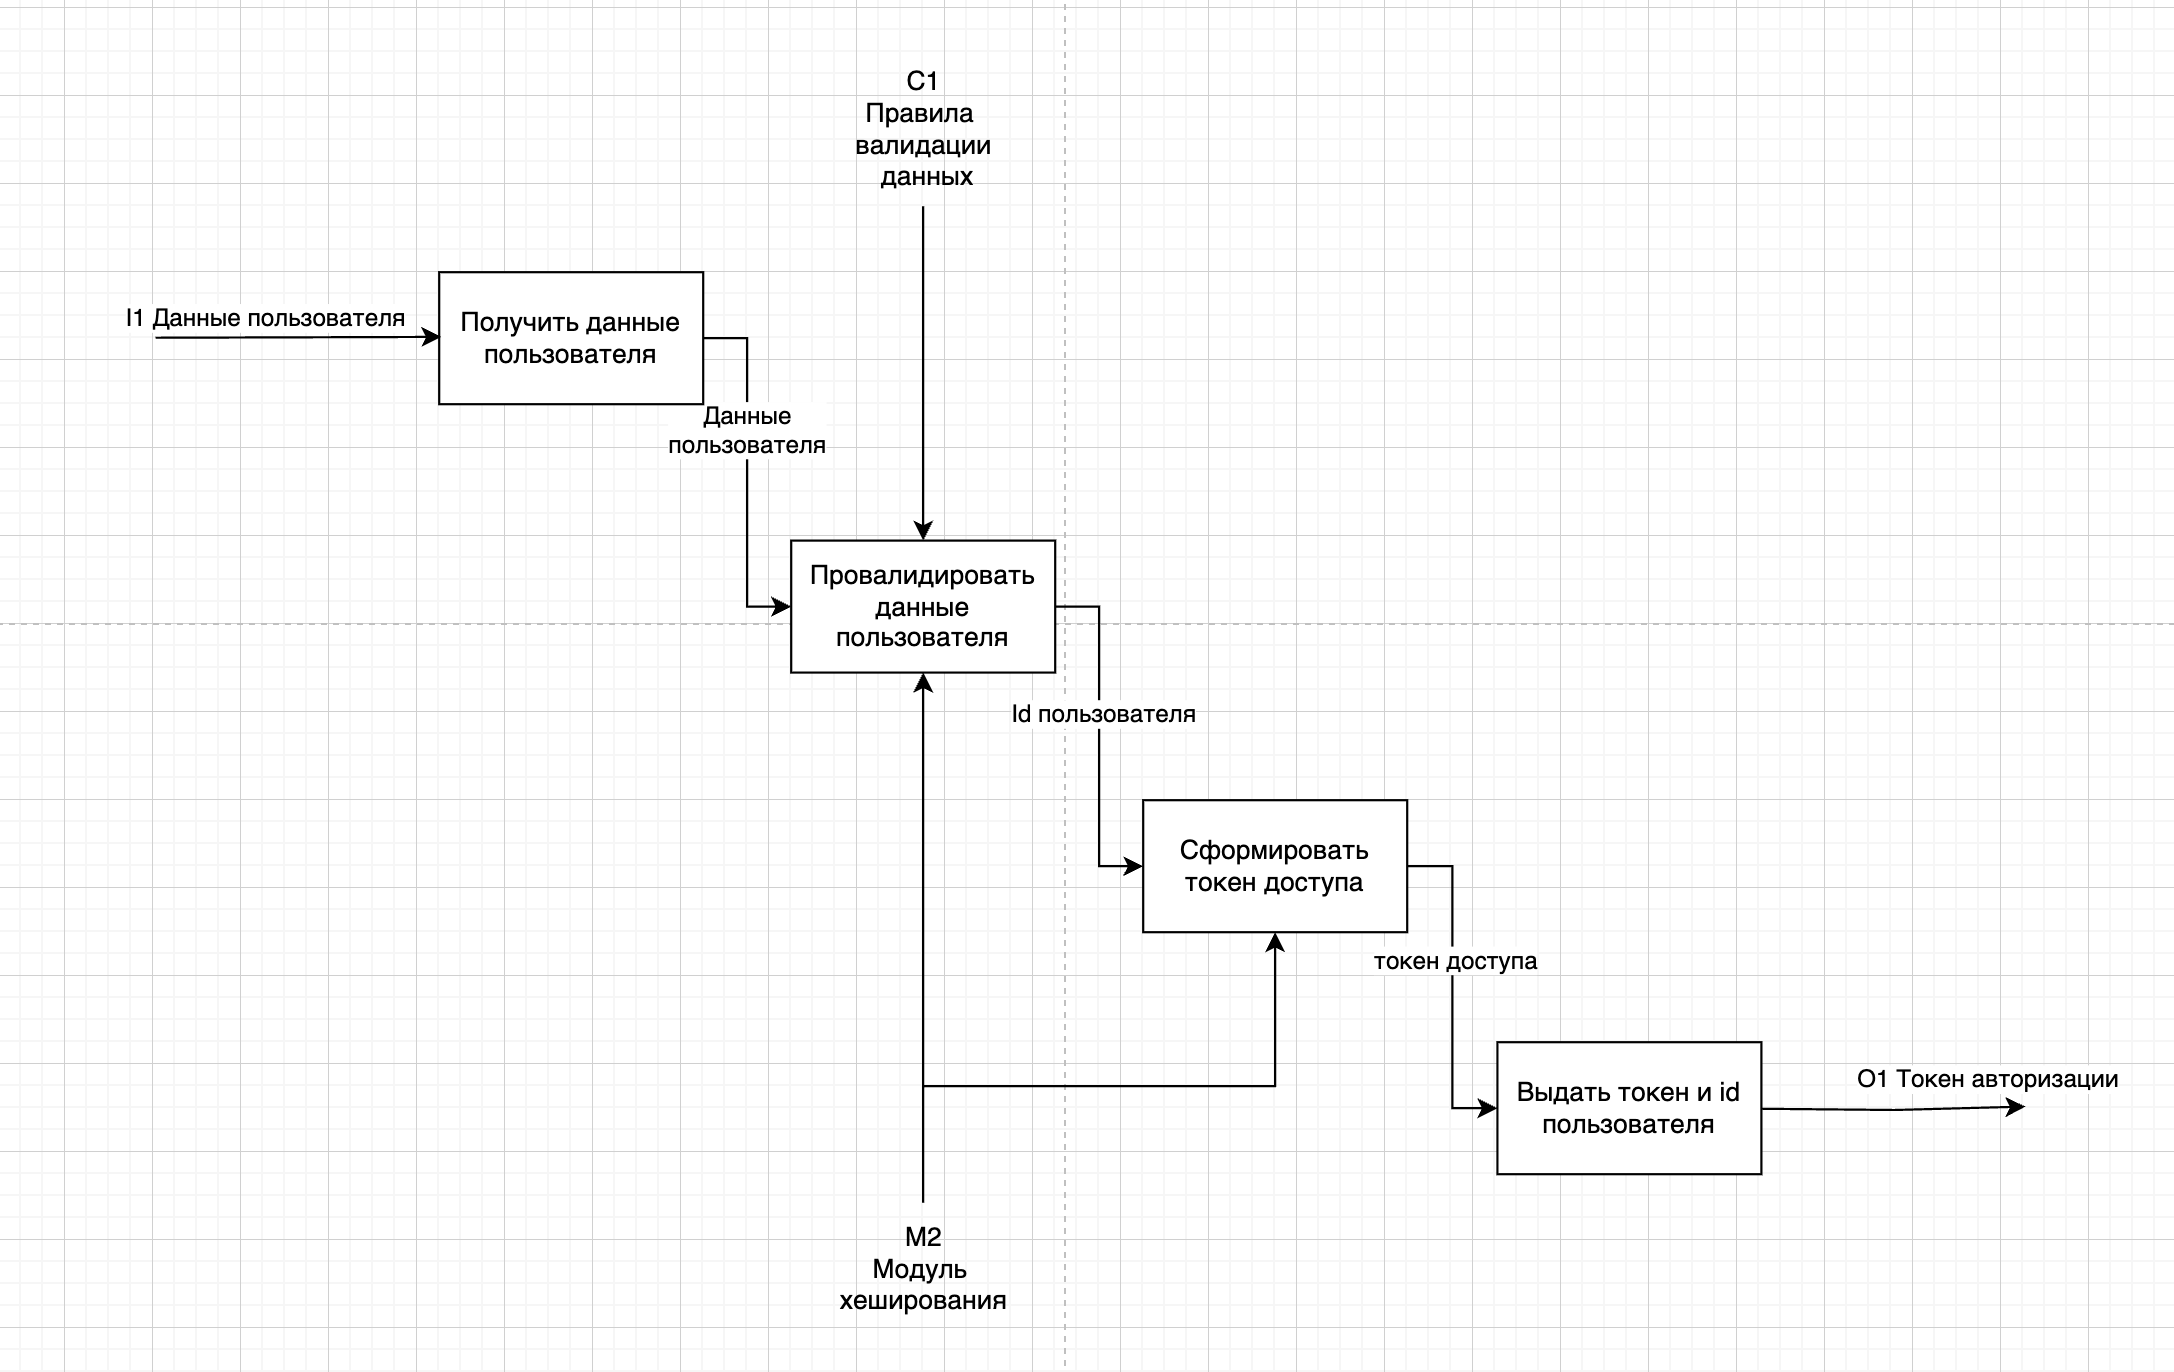
\includegraphics[width=0.7\linewidth]{images/idef0/image5.png}
     \captionof{figure}{Процесс авторизации в нотации IDEF0.}
     \label{fig:enter-label}
 }
\newpage
\mysection{Разработка технической части}

\mysubsection{Анализ техническийх требований}
\mysubsection{Проектирование базы данных}

На рисунке 16 представлена общая даталогическая модель базы данных. Она включает в себя 12 таблиц и описывает связи между ними.


{
    \centering
    \fbox{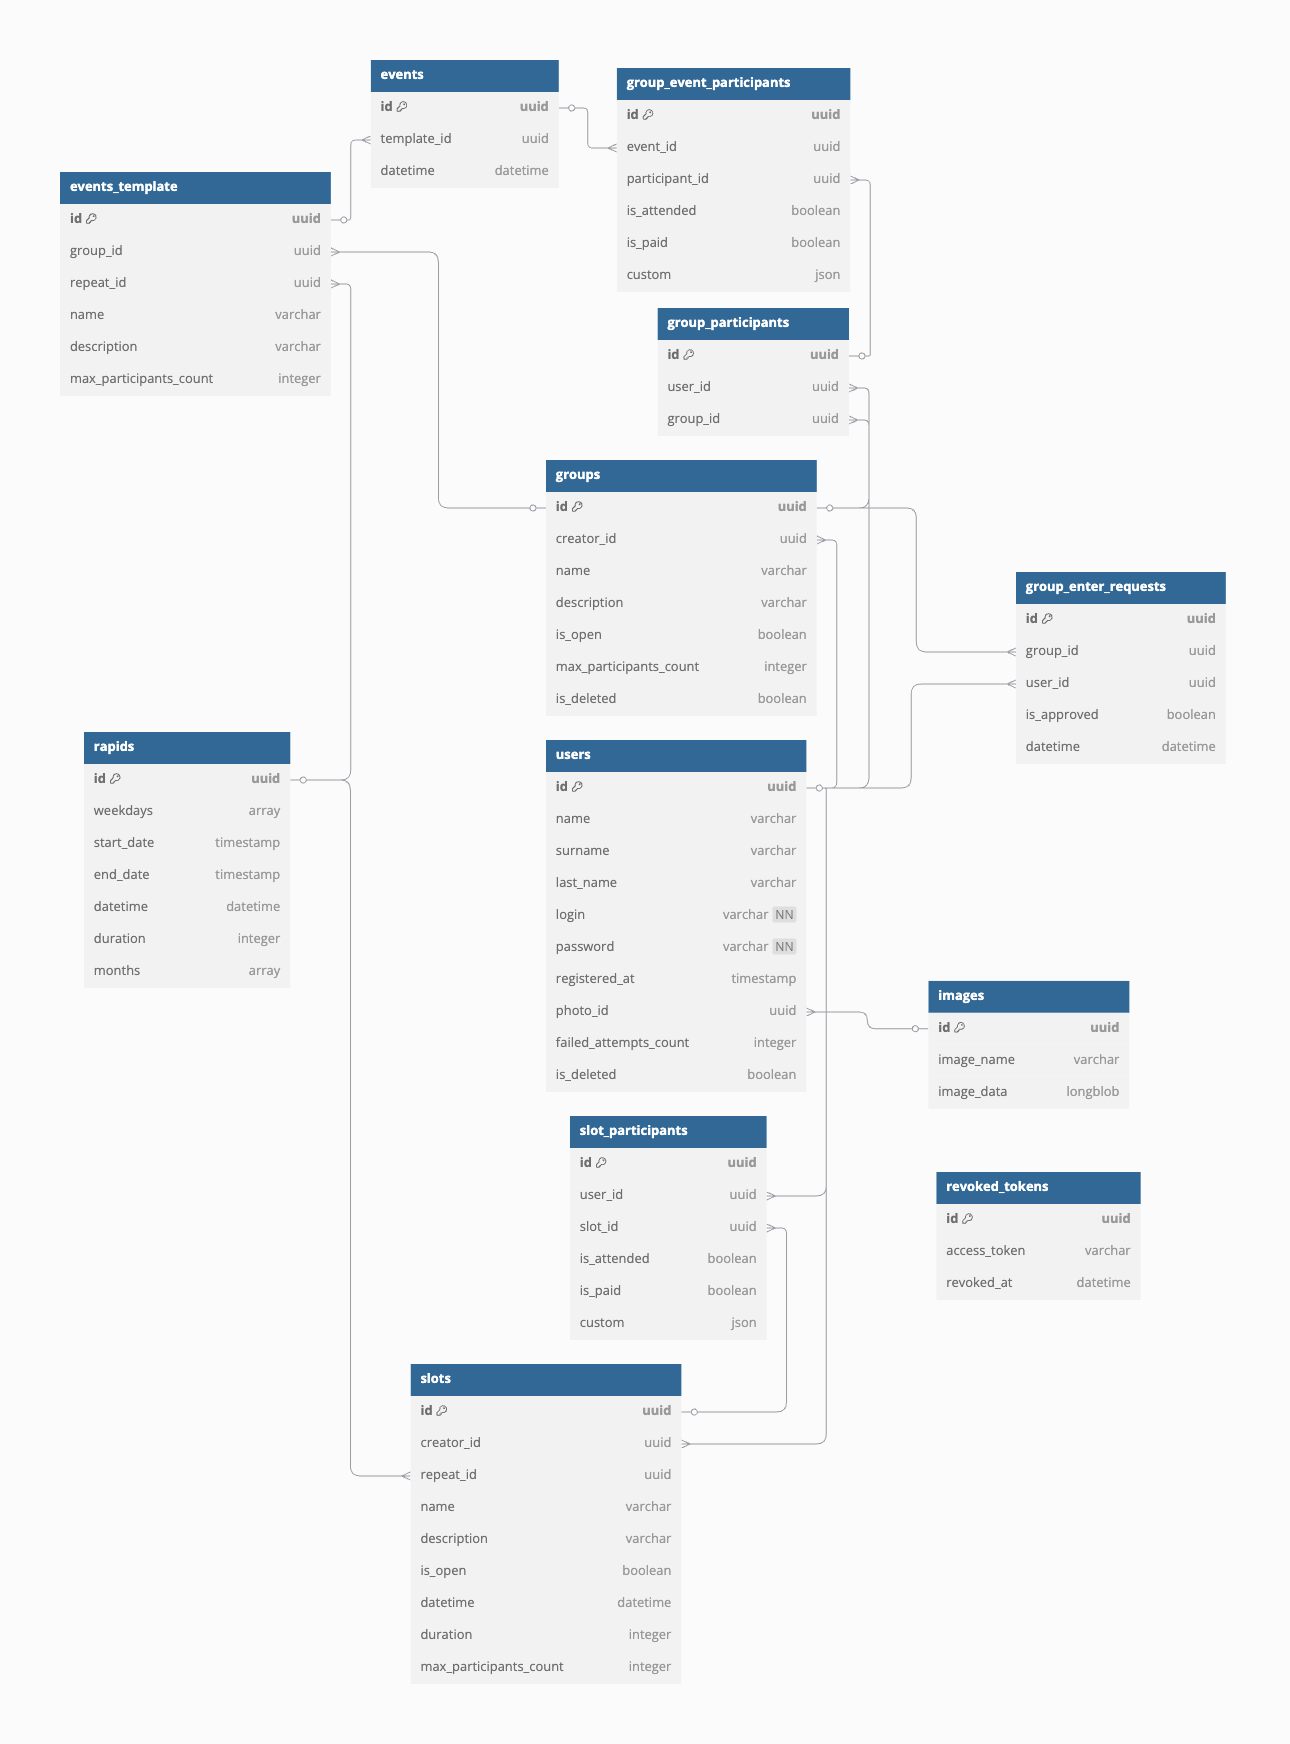
\includegraphics[width=0.5\linewidth]{images/DataBase.png}}
    \captionof{figure}{Схема реляционной базы данных}
    \label{fig:enter-label}
}

\myparagraph{Таблица о пользователях users}

Основными точками входа в эту таблицу являются поля
\begin{itemize}
    \item login - уникальное поле;
    \item password - хешированный пароль;
    \item photo\_id - идентификатор фотографии;
\end{itemize}

\myparagraph{Таблица об изображениях images}

Информация о картинках пользователей

\begin{itemize}
\item image\_name - название файла ;
\item image\_data - base64 формат картинки;
\end{itemize}

\myparagraph{Таблица о группах groups}

Группы могут быть закрытые и открытые, за это отвечает поле is\_open.

Все пользователи группы должны присутствовать на всех занятиях, которые создаются управляющим группы.

В открытые могут вступать все желающие, если есть места. 
В закрытые можно вступить, отправив запрос на вступление, который рассмотрит создатель группы.

\begin{itemize}
    \item creator\_id - id пользователя, который создал группу
\end{itemize}

\myparagraph{Таблица о запросах на вступление в группу group\_enter\_requests}


Поля таблицы:

\begin{itemize}
    \item user\_id - id пользователя, который отправил запрос  
    \item group\_id - id группы, в которую пользователь хочет вступить  
    \item datetime - дата и время создания запроса
    \item is\_approved - флаг о принятом или отклоненном запросе: 
\end{itemize}

\begin{itemize}
    \item По умолчанию NULL - запрос еще не рассмотрен
    \item True - запрос удовлетворен и пользователь заносится в таблицу 
    \item \text{group\_participants}
    \item False - запрос не удовлетворен
\end{itemize}

Администратор может изменить свое решение и принять участника в группу.

\myparagraph{Таблица об участниках групп group\_participants}

Пользователи могут состоять в нескольких группах.

\begin{itemize}
\item group\_id - id группы  
\item user\_id - id пользователя
\end{itemize}

\myparagraph{Таблица шаблонов событий events\_template}


Оригинал события или одного занятия, которое создает создатель группы. Он указывает описание и название занятия и частоту повторения.

\begin{itemize}
\itemgroup\_id - группа, в которой это событие происходит  
\itemrepeat\_id - ссылка на таблицу \texttt{rapids} с указанием частоты
\end{itemize}

\myparagraph{Таблица событий events}


Частные события, которые являются "наследниками" \texttt{events\_templates}.

Имеют характеристики того события, на которое указывает поле \texttt{template\_id}.  
\begin{itemize}
\itemdatetime - дата и время, в которое проходит конкретно это событие
\end{itemize}

Частные события создаются в момент начала занятия администратором группы. Когда администратор видит в интерфейсе, что у него по расписанию сейчас должно начаться занятие, он нажимает кнопку - создается конкретное занятие.

\myparagraph{Таблица об участниках событий group\_event\_participants}


Информация об участниках одного конкретного события.

О каждом участнике ведется информация: присутствовал ли он, оплачено ли занятие или другие кастомные параметры.

\myparagraph{Таблица об открытых событий slots}


Функционал слотов. Схож с событиями, но минуется слой с группами. Каждый слот - одновременно и группа и занятие. Может повторяться. Пользователи могут вступить в открытый слот. В закрытый - только по приглашению создателя. У слота указана частота повторения (может быть единожды).

\myparagraph{Таблица об участниках открытых событий slot\_participants}


Информация об участниках одного конкретного слота. Идет лишь ссылка по slot\_id к slots чтобы указать наследник какого слота эта запись
    

\mysubsection{Описание и разработка необходимых компонентов системы}
В качестве основного языка программирования выбран Python. Для создания функционального веб сервиса выбран фреймворк FastAPI. Он обеспечивает гибкий подход к реализации бизнес логики, поддерживает работу с реляционныыми SQL базами данных, а также гибок в настройке HTTP сервиса.

В качестве базы данных очевидным выбором стал PostgreSQL - одинз из самых базовых и основных SQL хостов на данный момент.

В слое CRM я выбрал sqlAlchemy - модельных архитектурный подъод, в котором каждая таблица в базе данных представлена моделью с которой работает система. Это обеспечивает разделение приложения на контекстные слои 

Вставить картинку слоев api routes validation models sql

На слое валидации я использую схемы от модуля pydentic. В отличии от openapi мне не нужно описывать входные и выходные параметры в yaml файлах, вся валидация происходит в специальных классах - схемах где указываются типы полей и pydentic схема сама валидирует введенные и возвращаемый параметры данных.

В качестве системы контроля версий был выбран github.

В качестве системы деплоя были выбраны Docker контейнеры, обеспечивающий быстрый запуск приложения в режиме разработки и в режиме выпуска продакшн версии продукта. Достаточно описать команды для деплоя докер контейнеры, так все необходимые файлы попадут в контейнер.
\mysubsection{Разработка необходимых вспомогательных компонентов для работы по HTTP}

\myparagraph{Описание алгоритмов}

На уровне API, первой точкой входа в систему на бекенде, являются так называемые end-поинты. Они являются публичными методами которые использует фронтенд часть проекта. 
Для оптимизации временных затрат я принял решение использовать POSTful API для того, чтобы не разделять логику процессов на риазличные типы запросов. Любое получение, изменение и создание сущностей в базе данных происходит через POST запросы. Они имеют закрытый body в формате JSON, обеспечивая поддержку любого типа данных ( будь это строки, числа, массивы или объекты)

В папке endpoints у меня лежат все файлы относящиеся к сущностям. Например, enter\_requests модуль отвечает за создание, чтение, удаление, а также за принятие и отклонение запросов на вступление в закрыте группы пользователей. 

Однако, с увеличением количества отдельных модулей возникает необходимость в оптимизации процесса добавления этих модулей в \_\_init\_\_ файл. Этот файл позволяет использовать все внутренниие файлы папки как один модуль, просто ссылаясь на папк endpoints. 

Для того чтобы избежать ручной ввод путей в этот инит файл, а также чтобы отловить все возможные ошибки внутри ендпоинтов и крудов, которые используются внутри них и не дать приложению не запуститься в принципе, я разрботал алгоритм, интегрирующий роутеры каждого ендпоинта в один общий роутер используемый FastAPi приложением. Этот алгоритм представлен на листинге 1.

\begin{lstlisting}[language=Python, caption=Алгоритм сбора маршрутов,breaklines=true, numbers=left]
"""
Entry point for all endpoints
"""

import os
import importlib
from fastapi import APIRouter
from env_constants import BASE_URL

app_router = APIRouter()


def include_routers(app_router: APIRouter):
    endpoints_path = os.path.join(os.path.dirname(__file__), 'endpoints')
    for filename in os.listdir(endpoints_path):
        if filename.endswith('.py') and filename != '__init__.py':
            module_name = filename[:-3]
            try:
                module = importlib.import_module(
                    f'api.endpoints.{module_name}')
                if hasattr(module, 'router'):
                    app_router.include_router(
                        module.router, prefix=f'/{BASE_URL}', tags=[module_name])
                    print(f'{module} router is added')
            except Exception as e:
                print(f'Failed to include router from {filename}: {e}')


include_routers(app_router)

\end{lstlisting}

Если разобраться более детально, что конерктно здесь происходит, то можно выделить следующее:

Перед тем как вызвать функцию агрегации маршрутов API я создаю общий FASTApi роутер в который буду добавлять все роутеры из модулей в папке edpoints.

Первым делом получаю абсолютный путь к папке в которой хранятся все наши ендпоинты (папка edpoints) с помощью встроенной библиотеки os (строка 14)

Далее итерируюсь по списку файлов внутри директории ендпоинтов (строка 15)

В случае если имя файла содержит \_\_init\_\_ - пропускаю этот файл и двигаюсь дальше (строка 16)

Далее с помощью бибилотеки importlib я динамически загружаю содержимое файла в оперативную память (строка 19). В случае если в модуле содержится переменная router, я включаю его в свой общий роутер. Таким образом, область включения маршрутов включает в себя все существующие маршруты без необходимости вручную импортировать их в общий инит файл.

Далее, в случае если один из роутеров содержит в себе ошибку, сработает обработчик Exception (строка 25) и выведет в консоль трейс ошибки и причину по которой маршрут не смог собраться. 

Далее в приложении уже используется обще собранный роутер со всеми рутами к ендпоинтам.
\mysubsection {Юнит-тестирование}
\mysubsection{Разработка интерфейса}

На рисунке 17 представлен макет страницы для входа в систему. Это форма с двумя полями, у каждого поля для ввода есть подсказки, а также указаны ошибки если введенные значения некорректны. Также, поле для ввода имеет глазик для предпосмотра введенного пароля.

{
    \centering
    \fbox{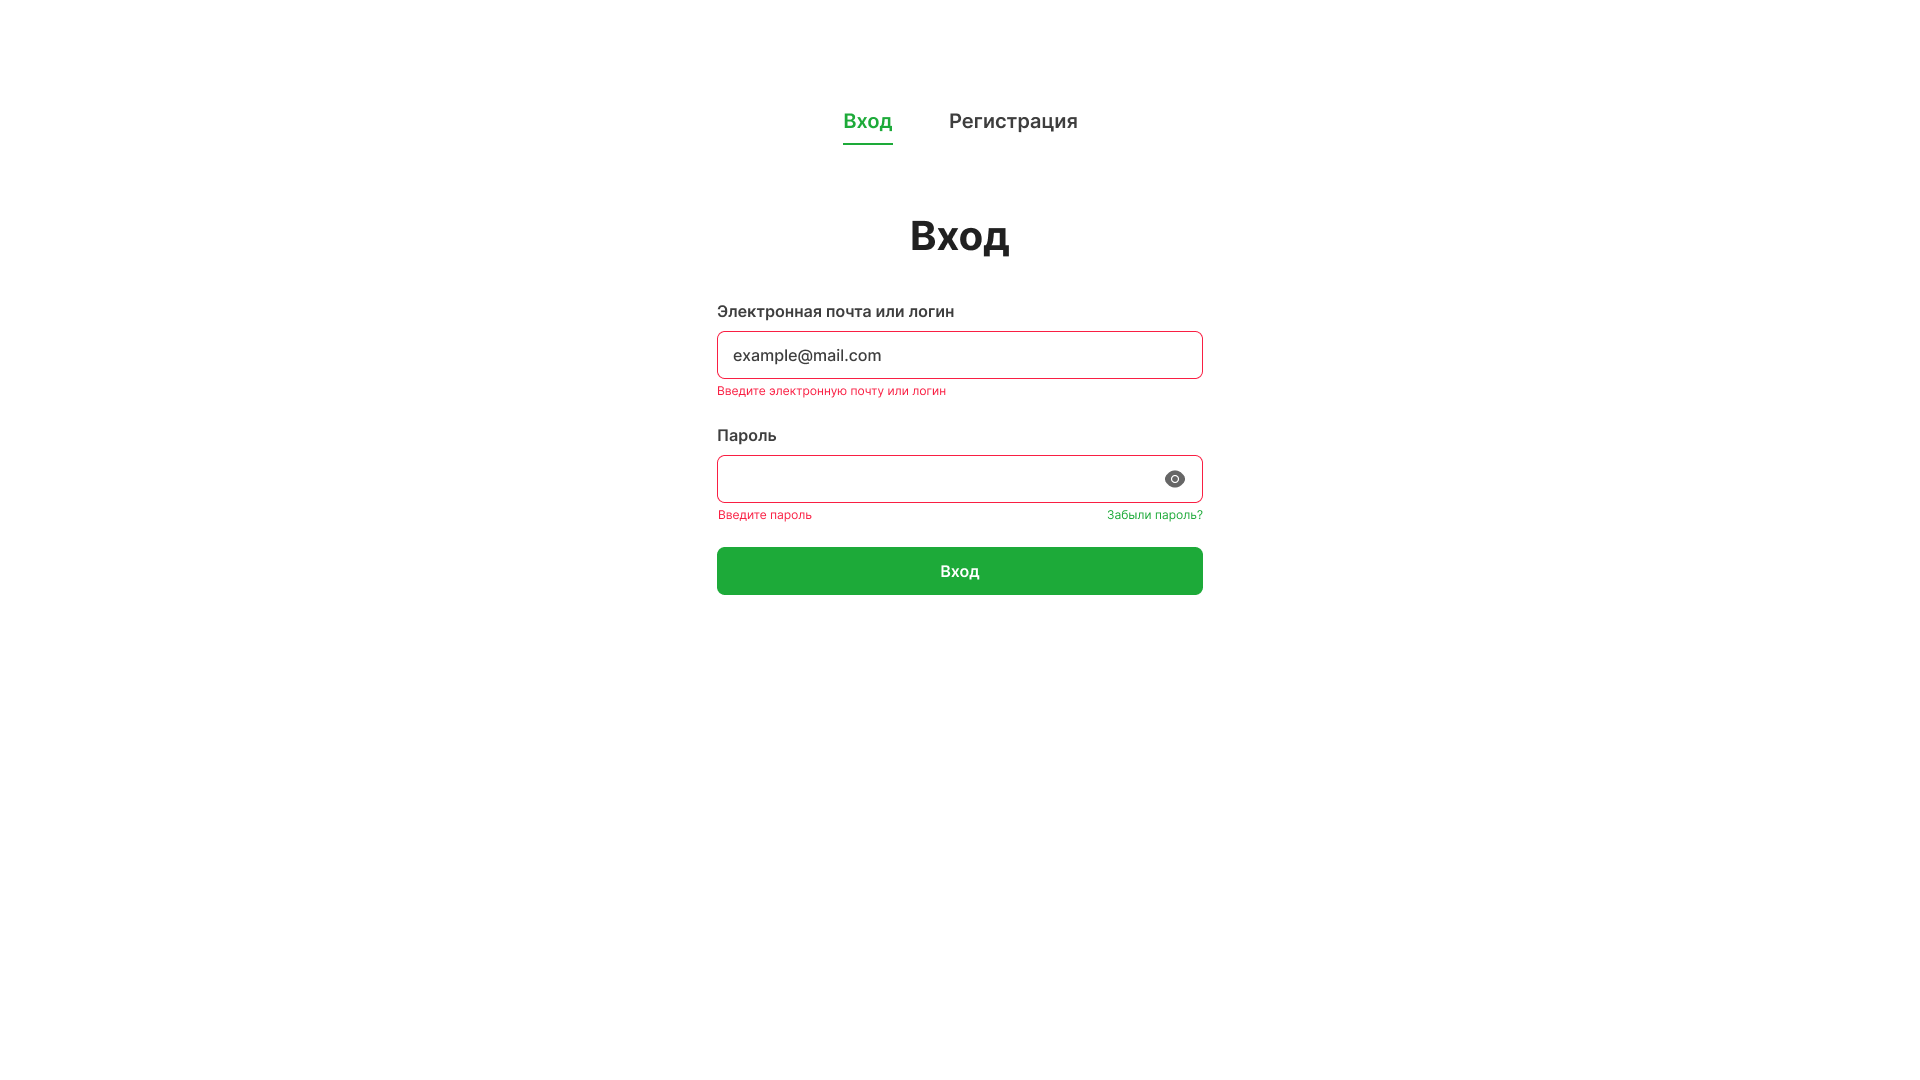
\includegraphics[width=0.7\linewidth]{images/design/Вход.png}}
    \captionof{figure}{Прототип страницы Вход}
    \label{fig:enter-label}
}

На рисунке 18 представлен макет страницы для регистарции в системе. В форме представлены основные поля необходимые лдя регистрации нового пользователя. При вводненесовпадающих пароей, высвечивается соответствующее сообщение о валидации. Также, под кнопкной о регистрации можно найти ссылку на условия обработки персональных данных.

{
    \centering
    \fbox{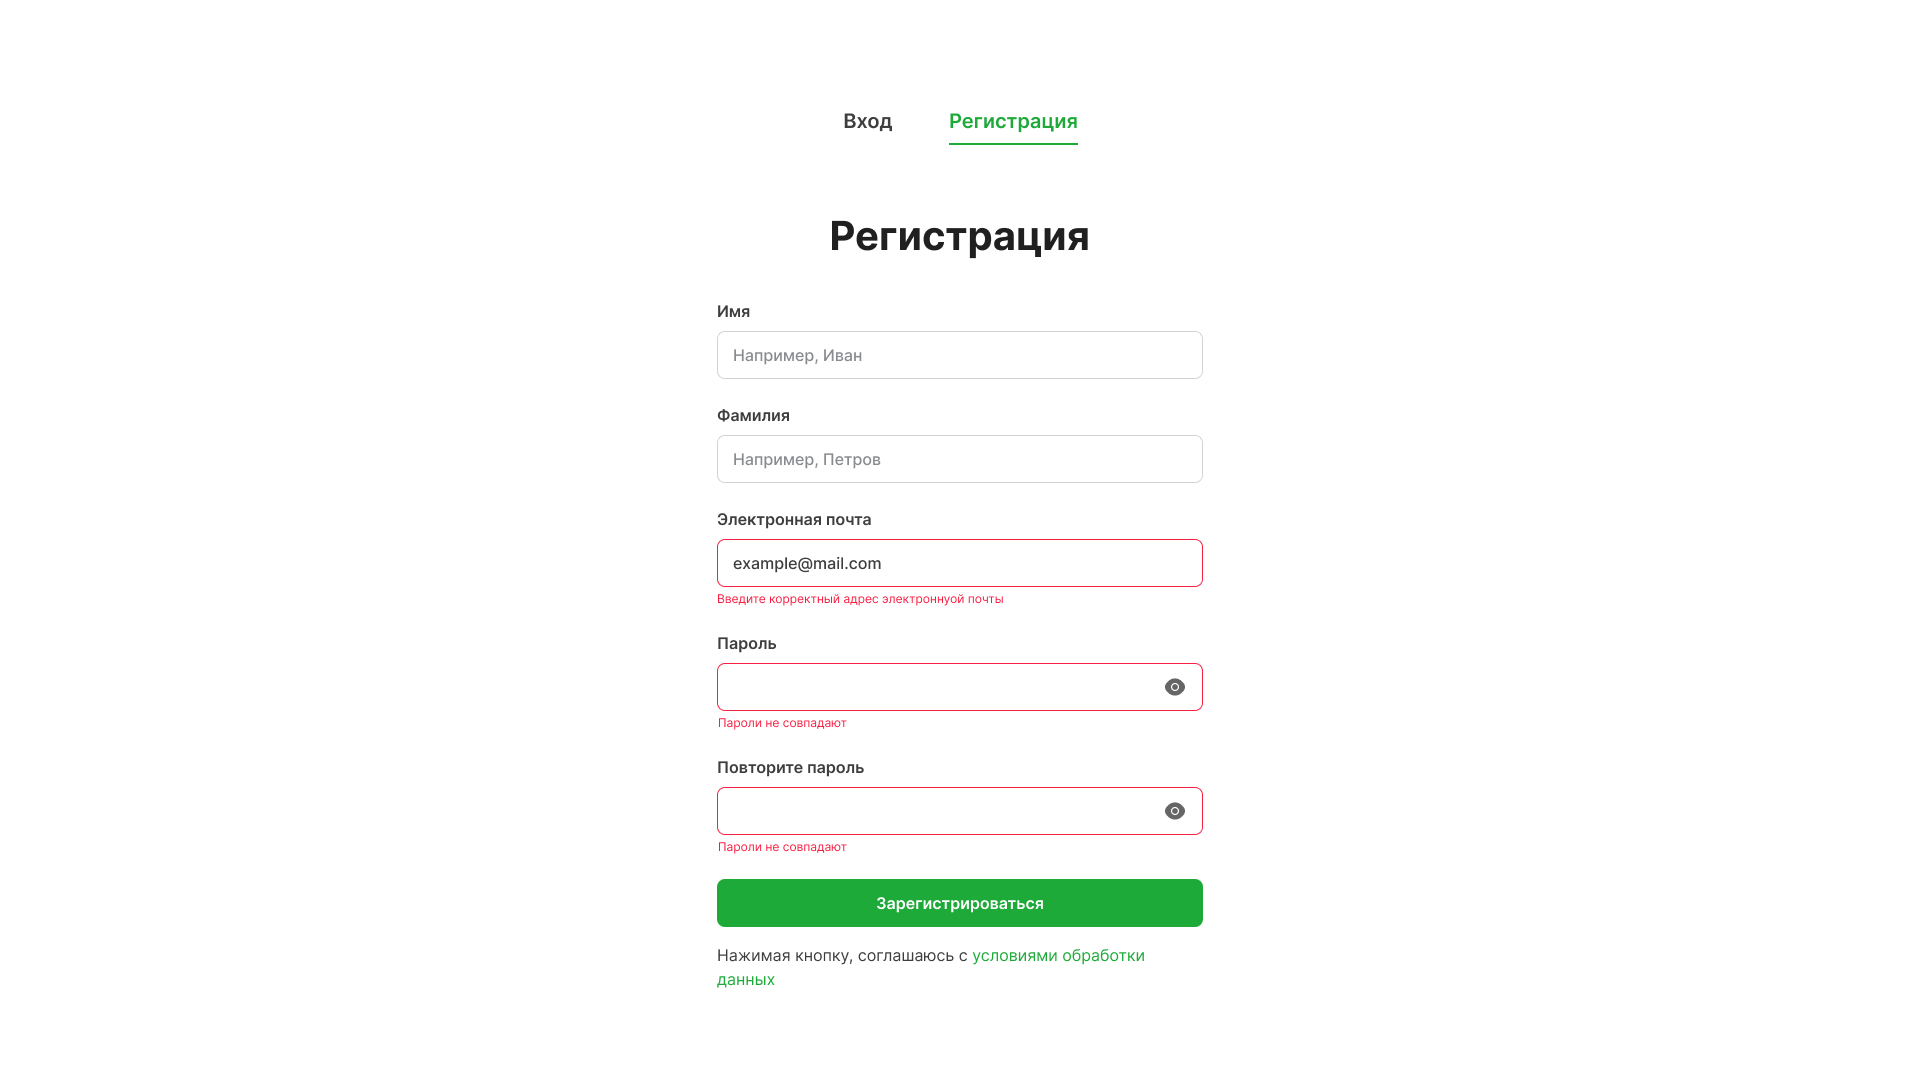
\includegraphics[width=0.7\linewidth]{images/design/Регистрация.png}}
    \captionof{figure}{Прототип страницы Регистрация}
    \label{fig:enter-label}
}

На рисунке 19 представлен макет страницы расписания пользователя - одного из 3 основных разделов сервиса. На вкладке расписание находится интерактивный компонент с календарем, позволяющий переключаться между месяцами, а также кнопкой создания занятия на выбранную дату. 

Справа от него находится более подробный компонент календаря с переключением между днем (рисунок 19), неделей (рисунок 20) и месяцем (рисунок 21). 

В каждом из них в удобном формате представлены предстоящие занятия среди всех групп.
\newpage
{
    \centering
    \fbox{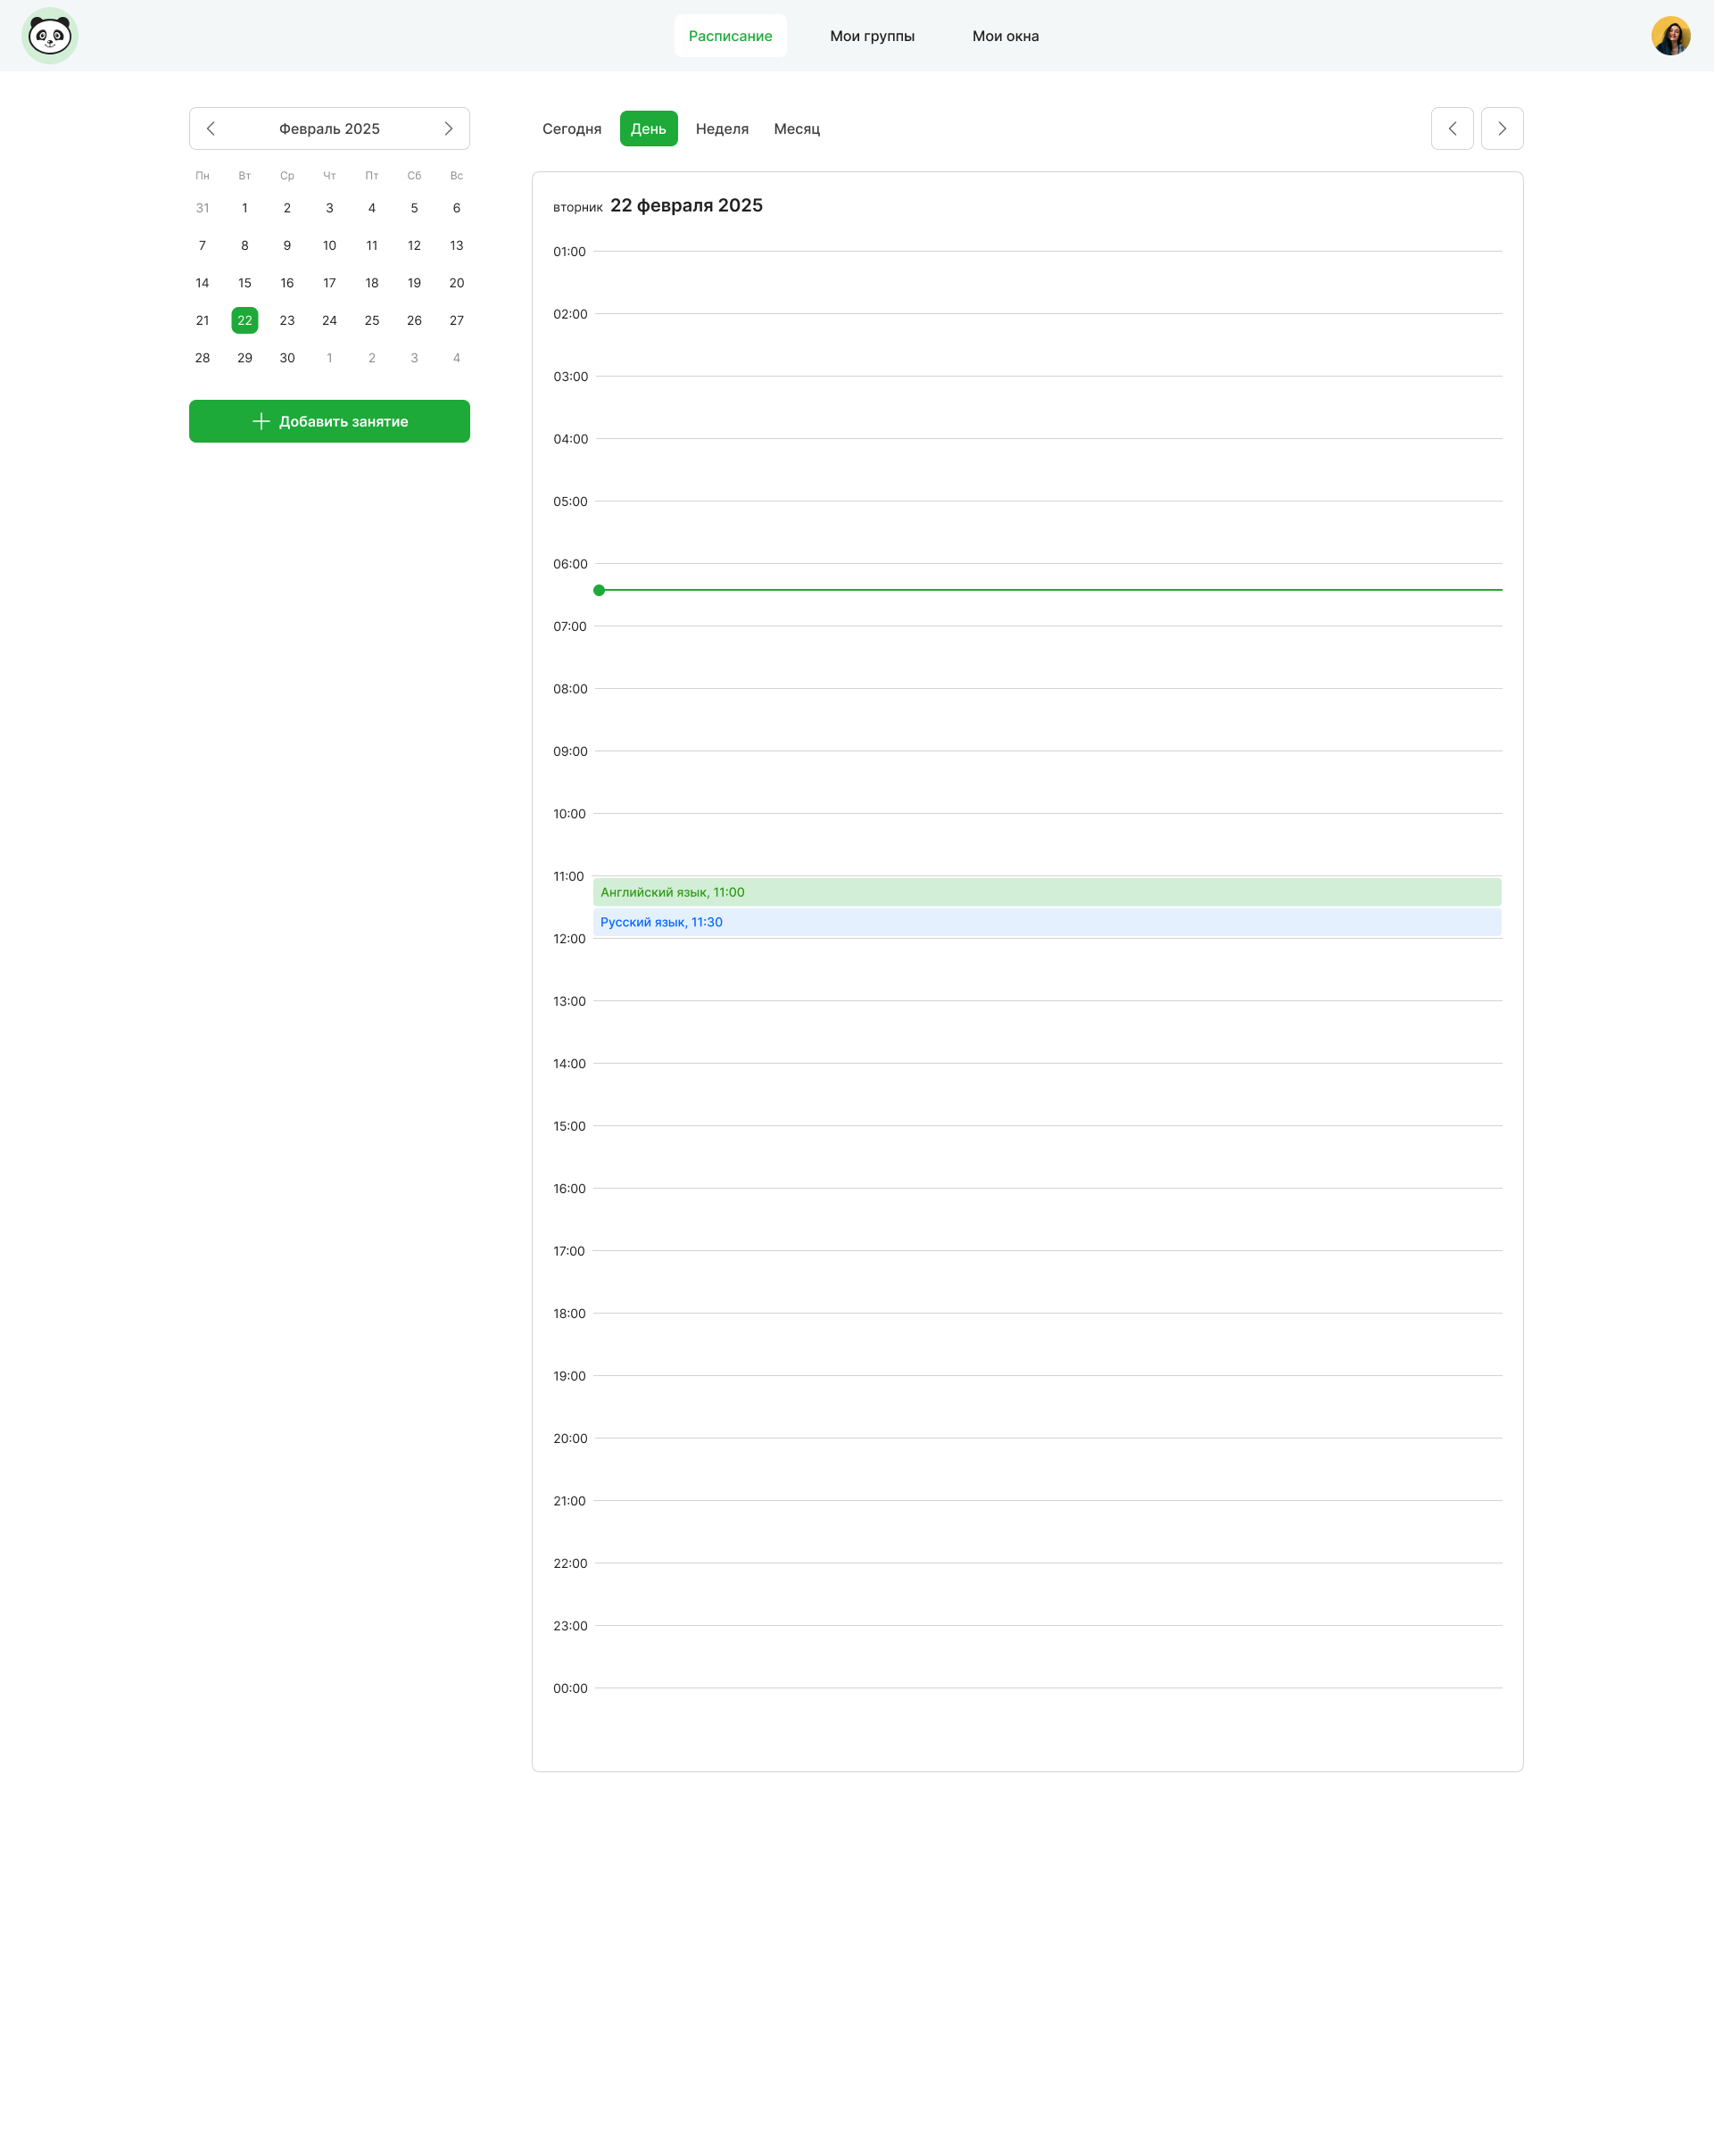
\includegraphics[width=0.7\linewidth]{images/design/Расписание_День.png}}
    \captionof{figure}{Прототип страницы "Расписание". Календарь, день}
    \label{fig:enter-label}
}


{
    \centering
    \fbox{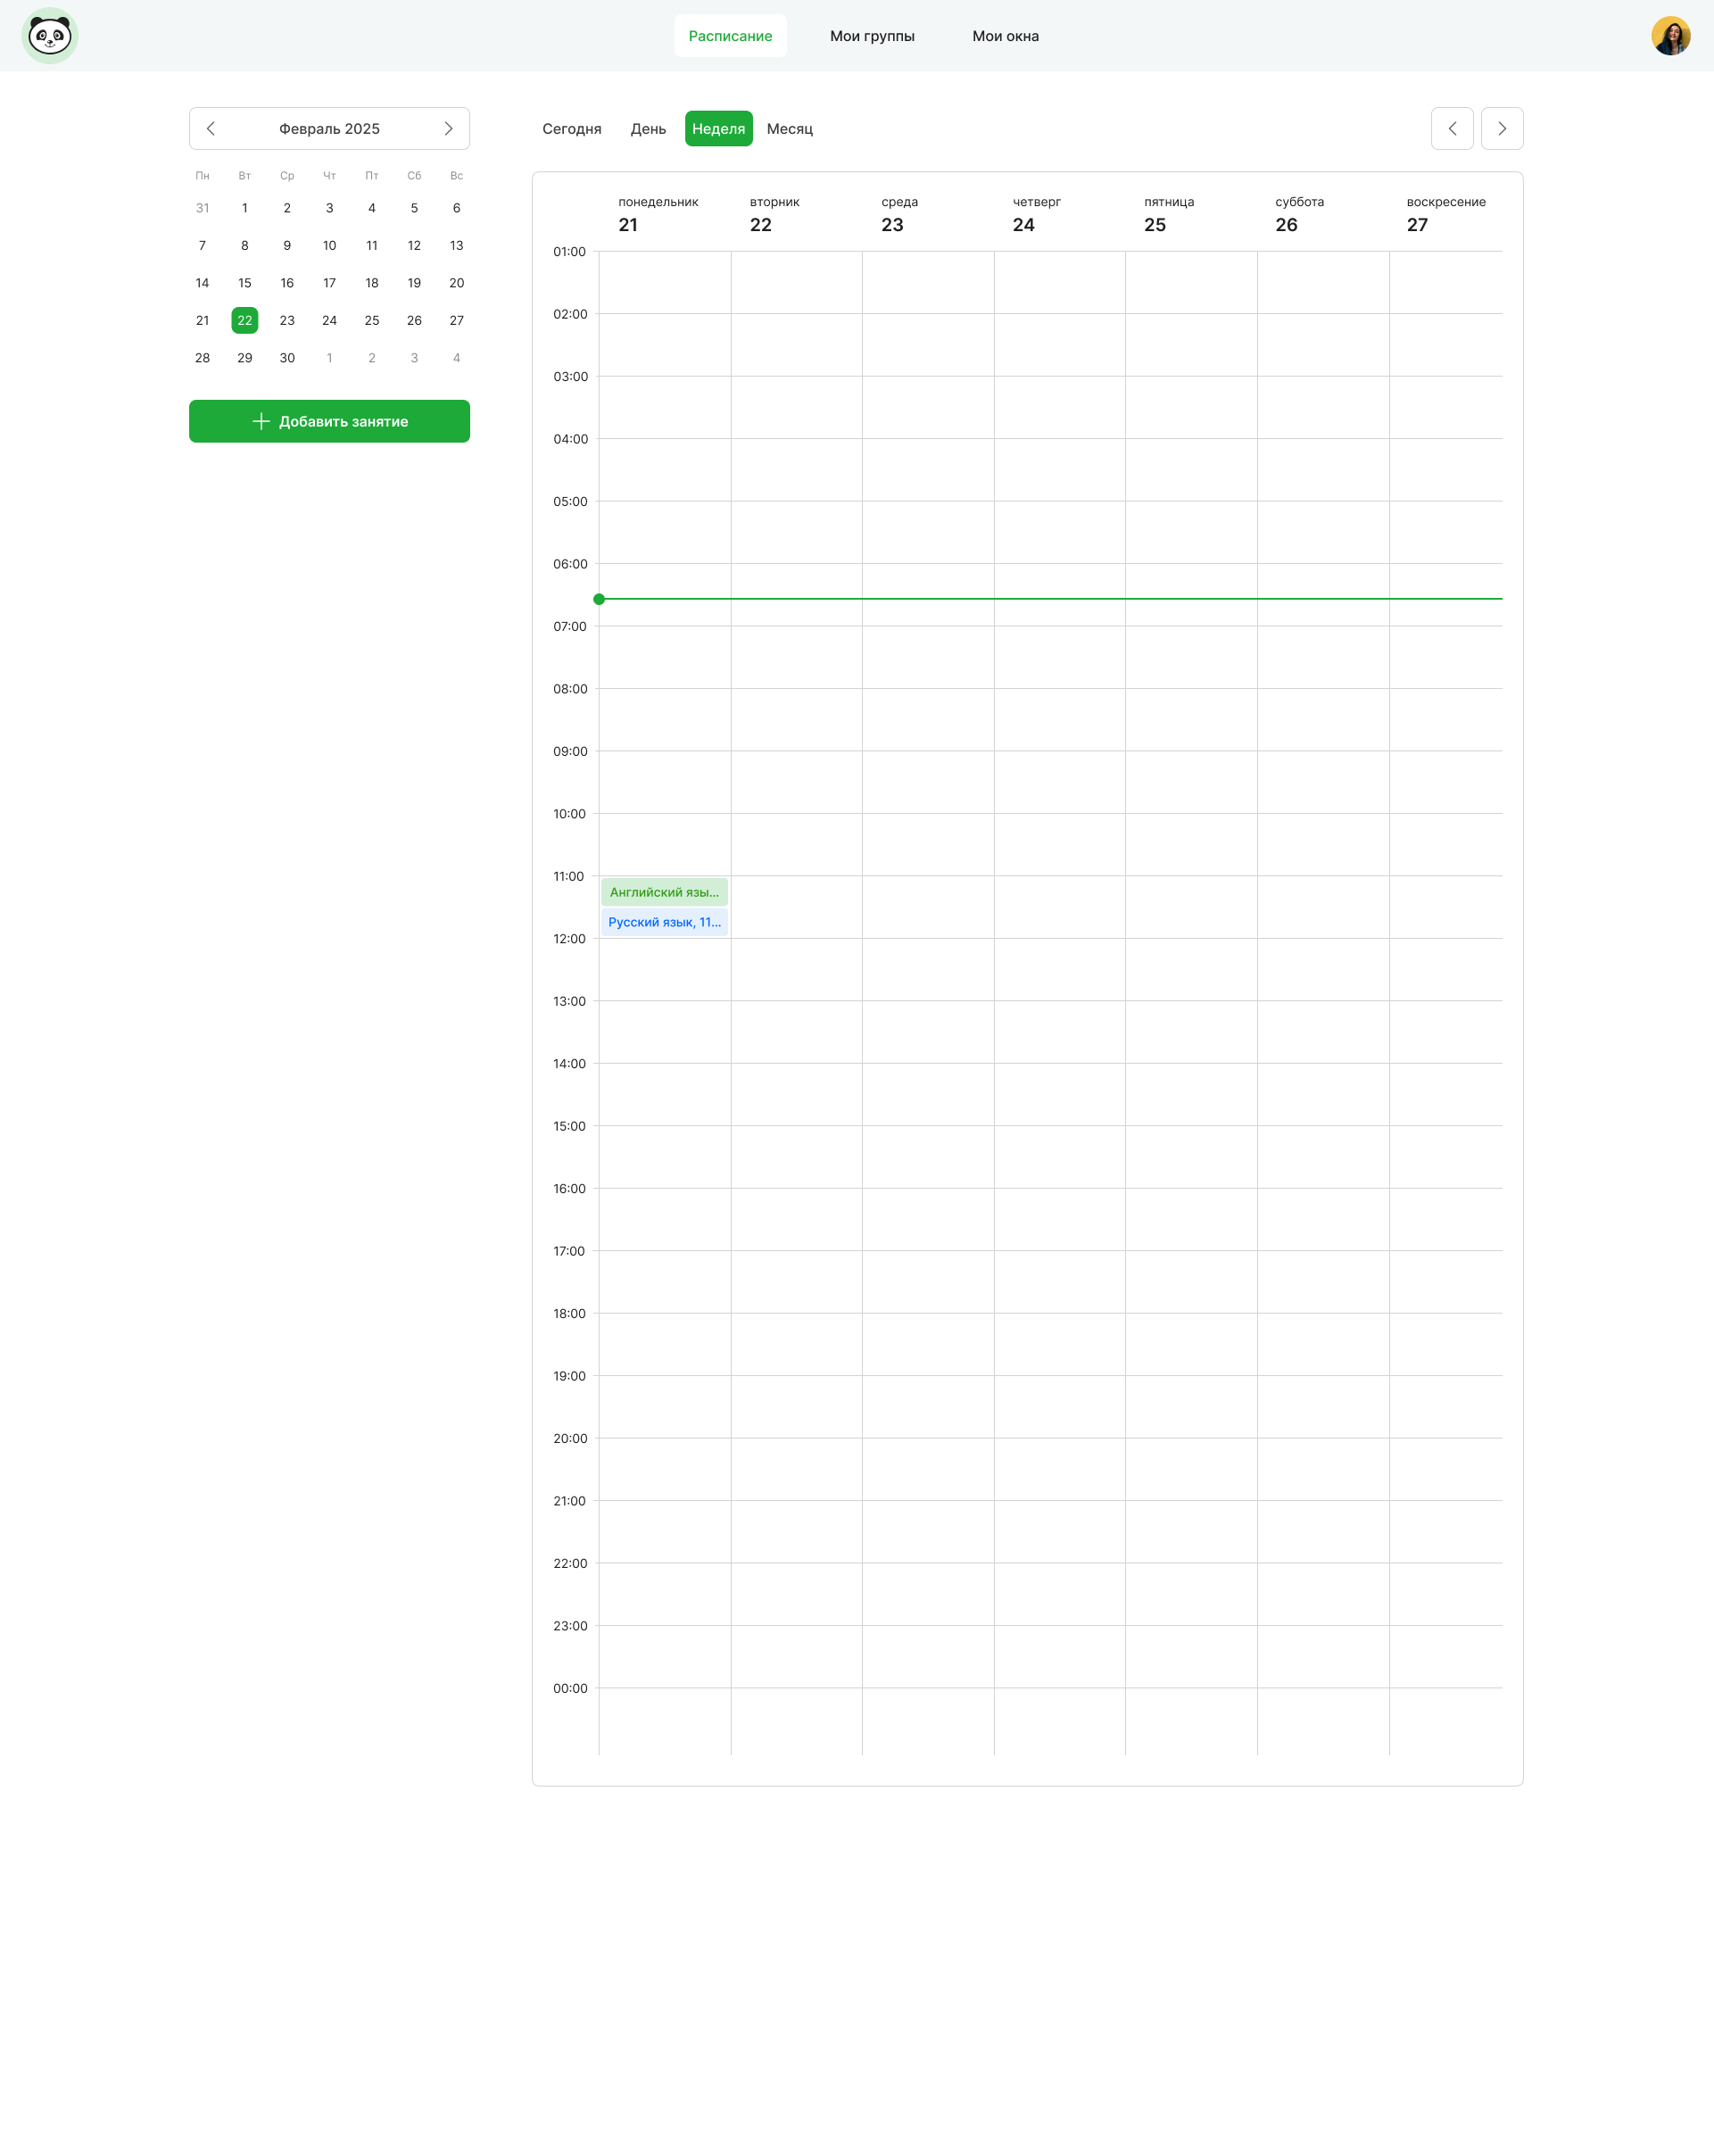
\includegraphics[width=0.5\linewidth]{images/design/Расписание_Неделя.png}}
    \captionof{figure}{Прототип страницы "Расписание". Календарь, неделя}
    \label{fig:enter-label}
}

{
    \centering
    \fbox{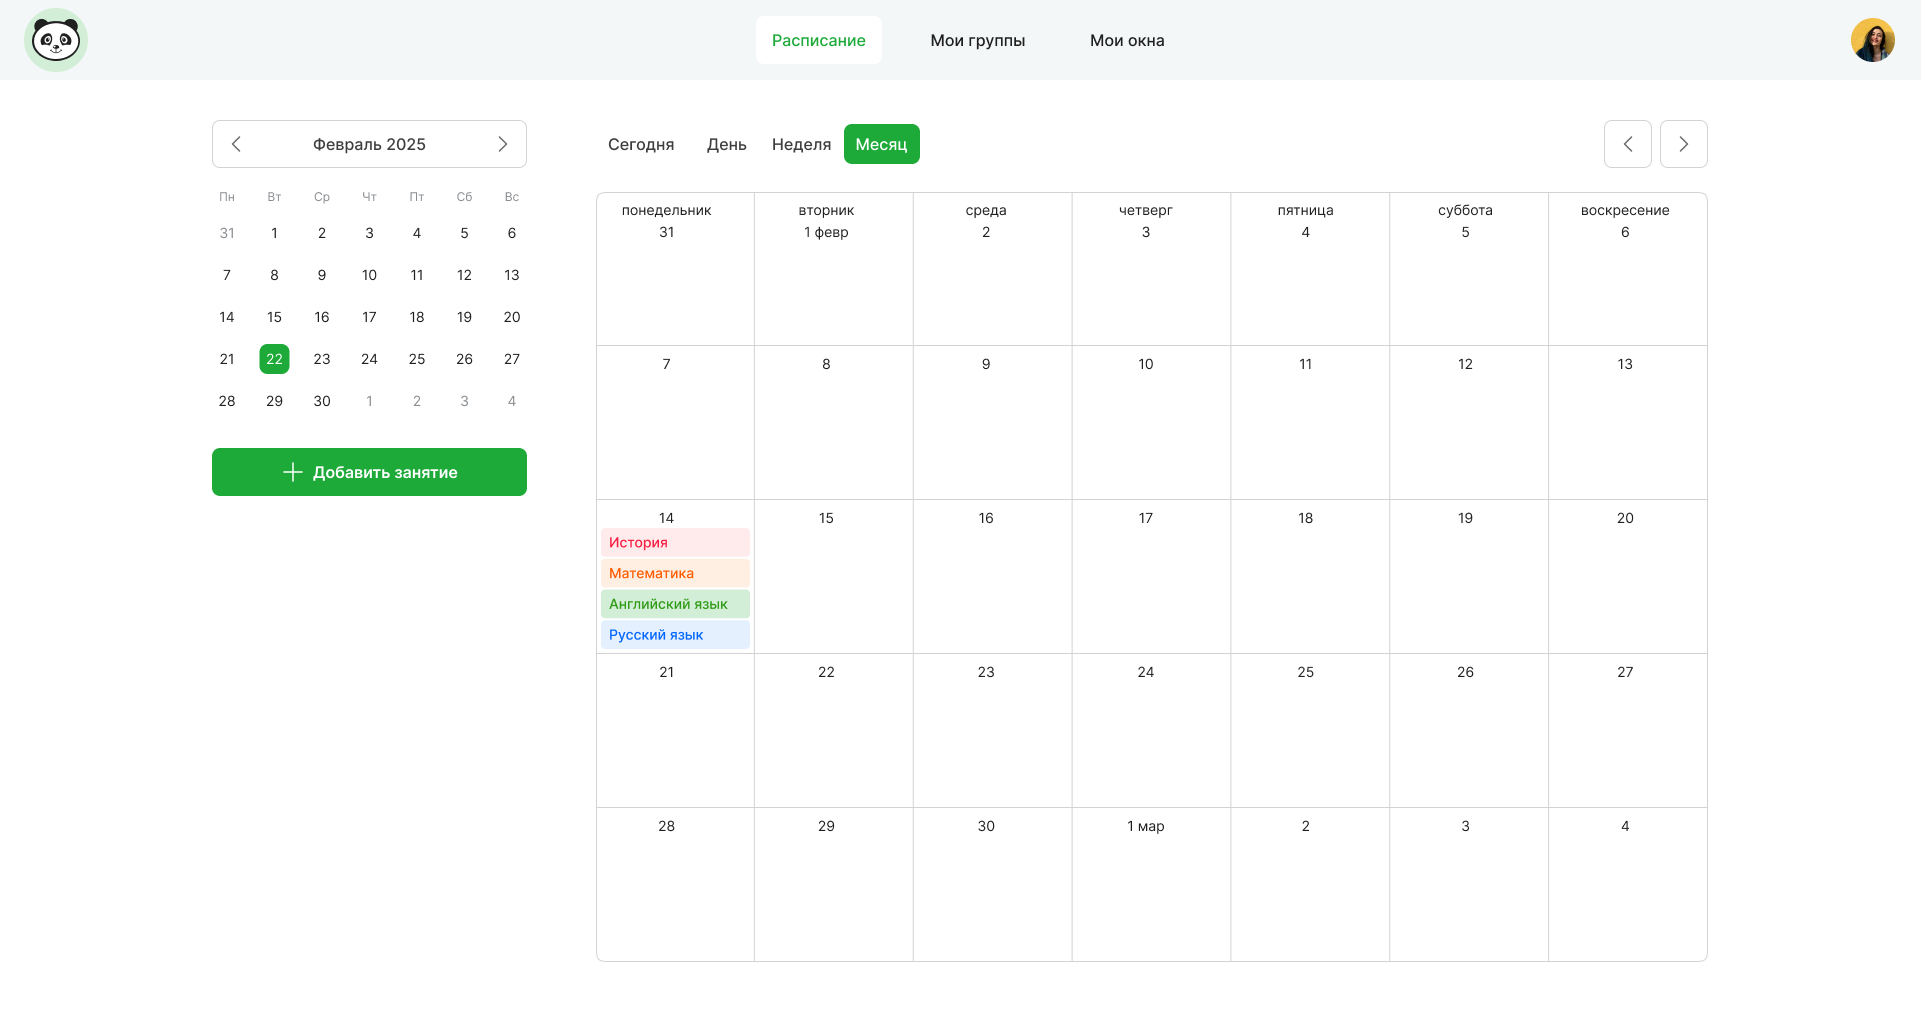
\includegraphics[width=0.7\linewidth]{images/design/Расписание_Месяц.png}}
    \captionof{figure}{Прототип страницы "Расписание". Календарь, месяц}
    \label{fig:enter-label}
}


\mysubsubsection { Создание уникальной айдентики сайта ( UI-kit)}

\mysubsubsection {Обзор внешнего вида всех компонентов, форм и таблиц}

\mysubsubsection {Прототипирование}


\mysubsection {Разработка веб-части}
\mysubsubsection {Поиск оптимального стека технологий необходимый для выполнения требований}
\mysubsubsection {Написание API}
\mysubsubsection {Разработка UI, обхих компонентов и базовой функциональности}
\mysubsubsection {Создание и наполнение страниц}
\mysubsubsection {Сращивание с бекендом}
\mysubsubsection {Интеграционное тестирование функционала}

\newpage
\mysection{Глава}
\mysubsection {Ввод системы в эксплуатацию}
\mysubsection {Сбор обратной связи и QA}
\mysubsection {Определения списка результатов по которым можно определить удовлетворенность пользователей}

\end{document}
